\chapter*{Geysers d’El Tatio\markboth{Geysers d’El Tatio}{}}
\section*{20 mars 2015}
Après Valparaiso plusieurs possibilités : continuer en vélo ou prendre un bus vers le nord. J'ai décidé d'aller directement à San Pedro de Atacama pour pouvoir bien profiter de toute la région nord du Chili, altiplano bolivien et sud du Pérou. 

 Je vais donc à la gare de bus de Valparaiso à 23h pour un trajet qui doit durer plus de 24h. Malheureusement je suis tombé sur un chauffeur un peu borné qui a refusé d'embarquer le vélo. Résultat une nuit de plus à Valparaiso et un départ le lendemain midi mais vers la ville de Calama à 100km de San Pedro.
\begin{center} 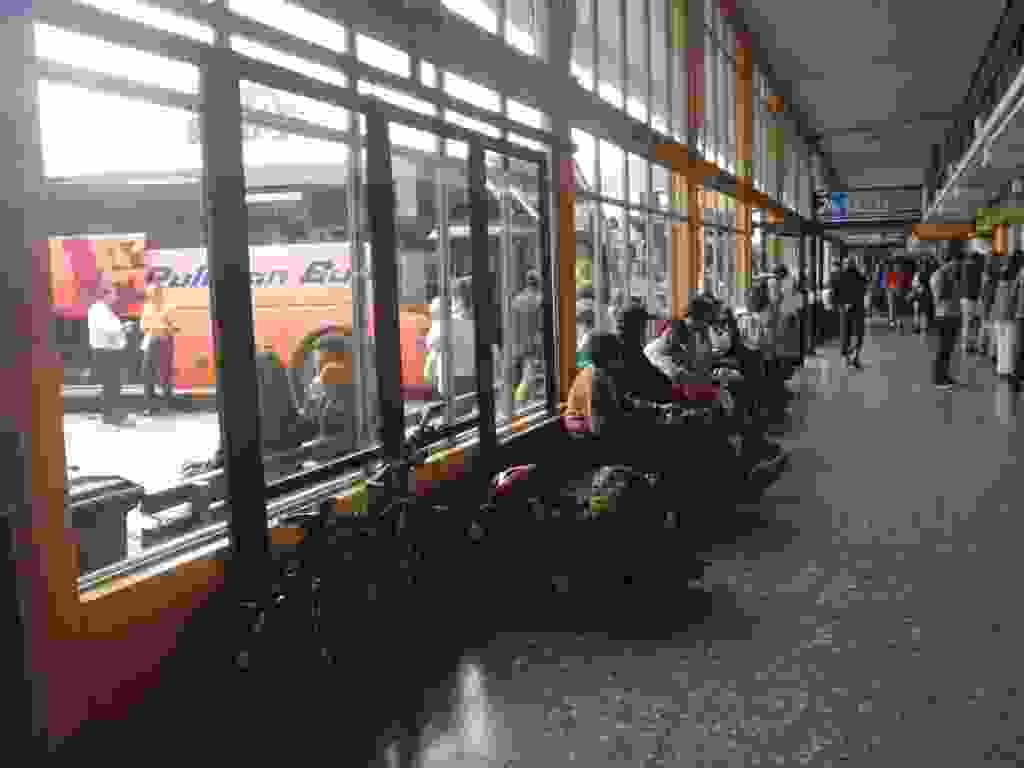
\includegraphics[width=\mywidth]{../wp-content/uploads/2015/03/P3122760-1024x768.jpg} \end{center}

 En remontant le vélo en arrivant, je vois que la roue arrière tourne difficilement : cette fois c'est le cône de roulement qui est usé, heureusement j'ai trouvé un magasin pour changer la pièce rapidement. Les réparateurs chiliens sont décidément efficaces !

 Calama, dans la région des mines de cuivre.
\begin{center} 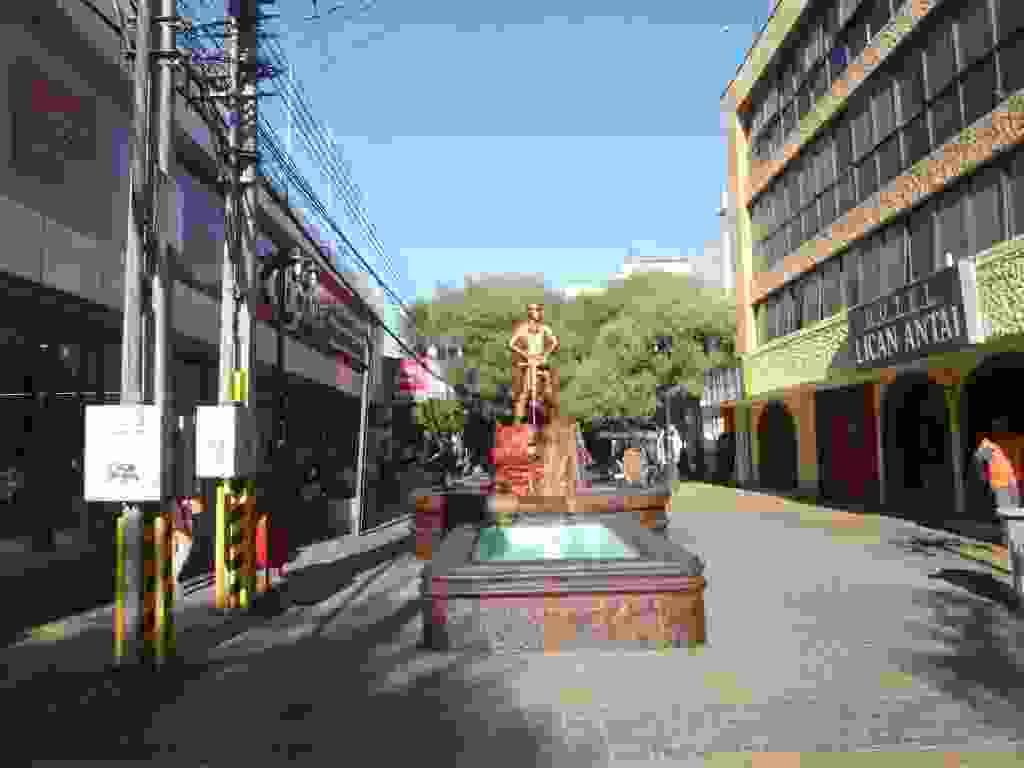
\includegraphics[width=\mywidthreduced]{../wp-content/uploads/2015/03/P3132768-1024x768.jpg} \end{center}

 Au lieu de prendre la route directe vers San Pedro, je profite d'être à Calama pour faire un détour par les geysers d'El Tatio. 

 C'est parti pour environ 5 jours en quasi autonomie, vélo bien chargé en nourriture et en eau, un bon test pour la suite en Bolivie. 

 La première partie traverse le désert.
\begin{center} 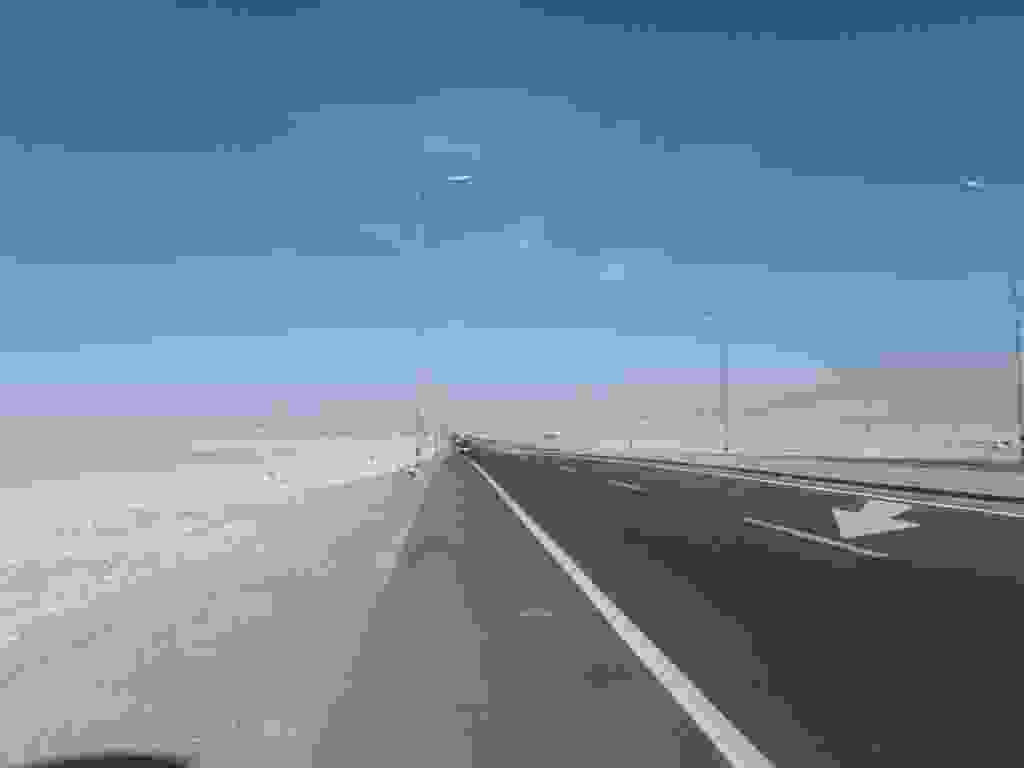
\includegraphics[width=\mywidthreduced]{../wp-content/uploads/2015/03/P3142773-1024x768.jpg} \end{center}
\vspace{-\topsep}

\pagebreak
~
\begin{center} 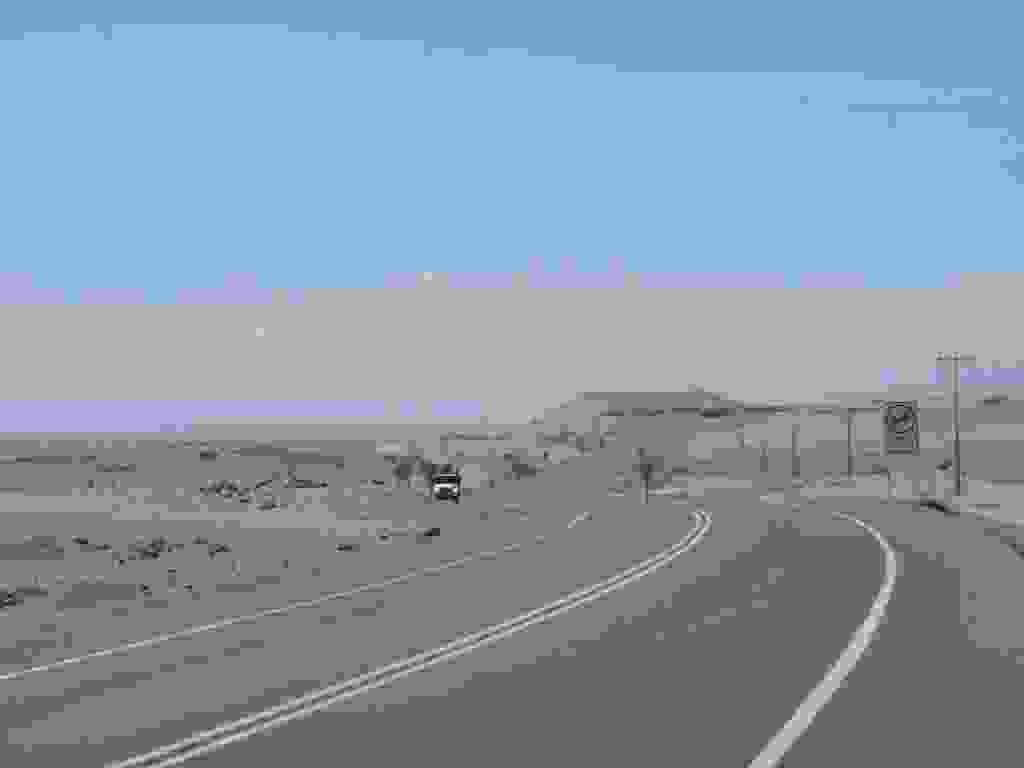
\includegraphics[width=\mywidth]{../wp-content/uploads/2015/03/P3142776-1024x768.jpg} \end{center}
\begin{center} 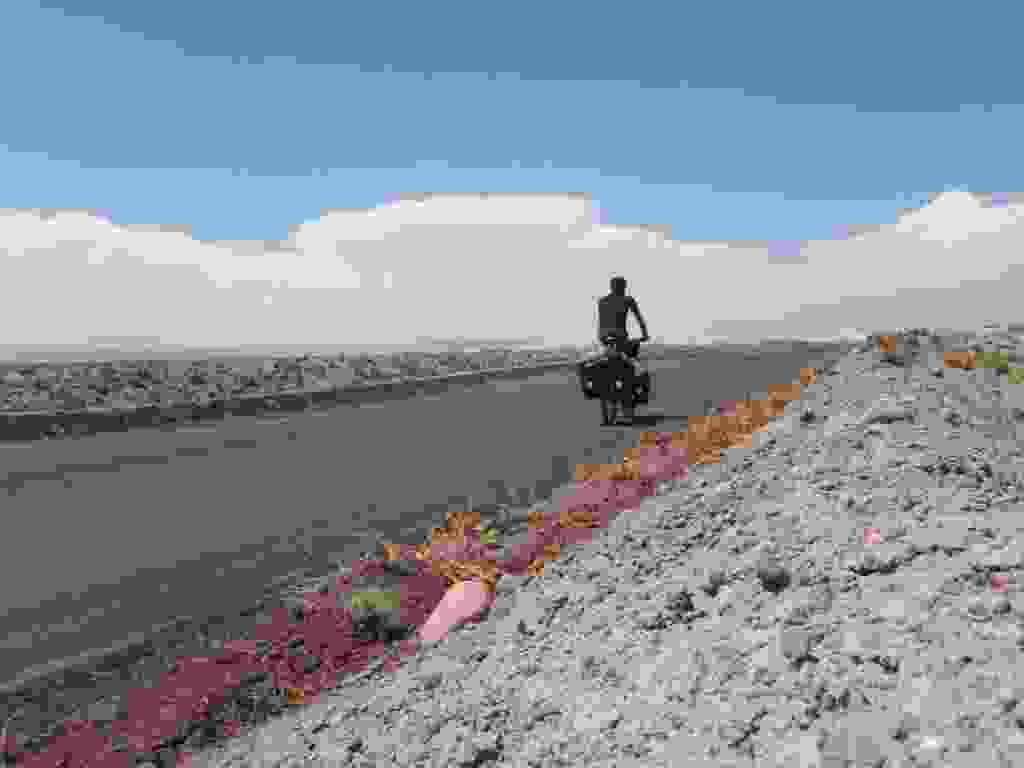
\includegraphics[width=\mywidth]{../wp-content/uploads/2015/03/P3142782-1024x768.jpg} \end{center}
\vspace{-\topsep}
\vspace{-3.25mm}

\pagebreak
Je passe par le village de Chiu Chiu.
\begin{center} 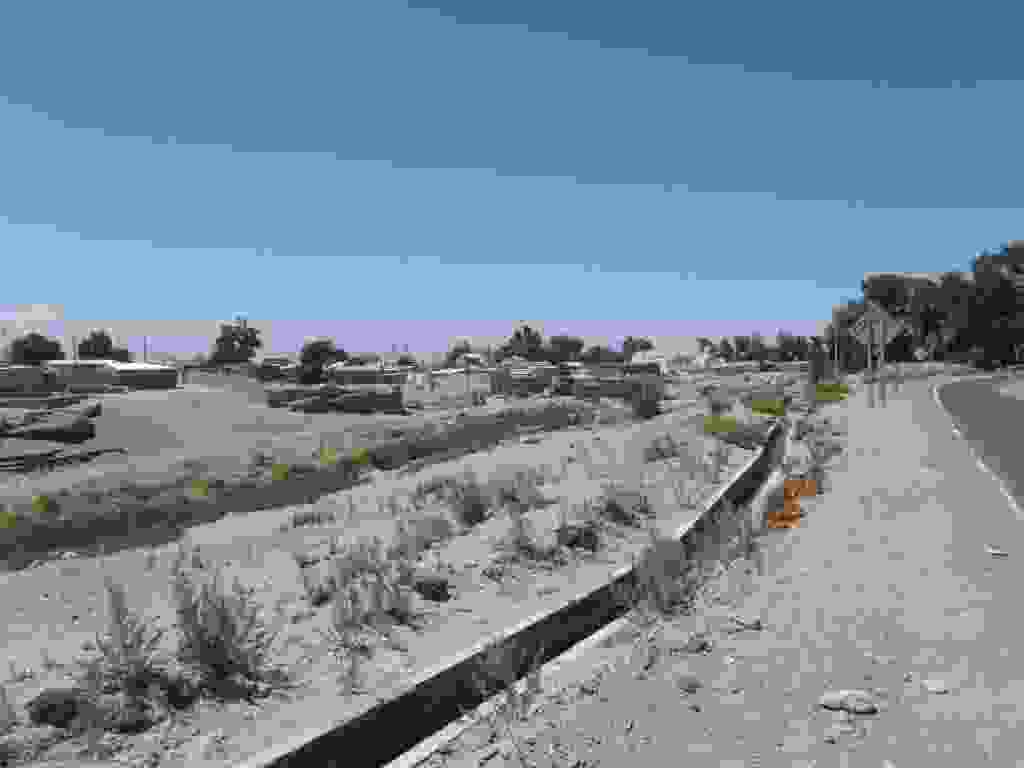
\includegraphics[width=\mywidth]{../wp-content/uploads/2015/03/P3142777-1024x768.jpg} \end{center}
\begin{center} 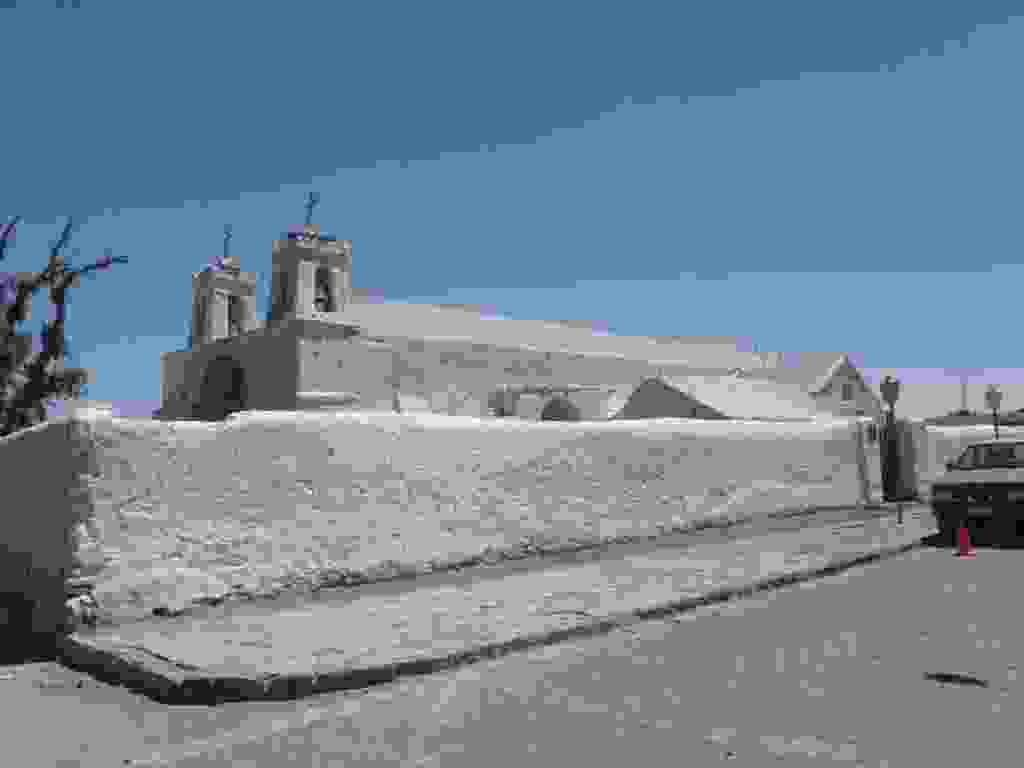
\includegraphics[width=\mywidth]{../wp-content/uploads/2015/03/P3142779-1024x768.jpg} \end{center}
\vspace{-\topsep}
\vspace{-3.25mm}

\pagebreak
Un petit lac au milieu du désert.
\begin{center} 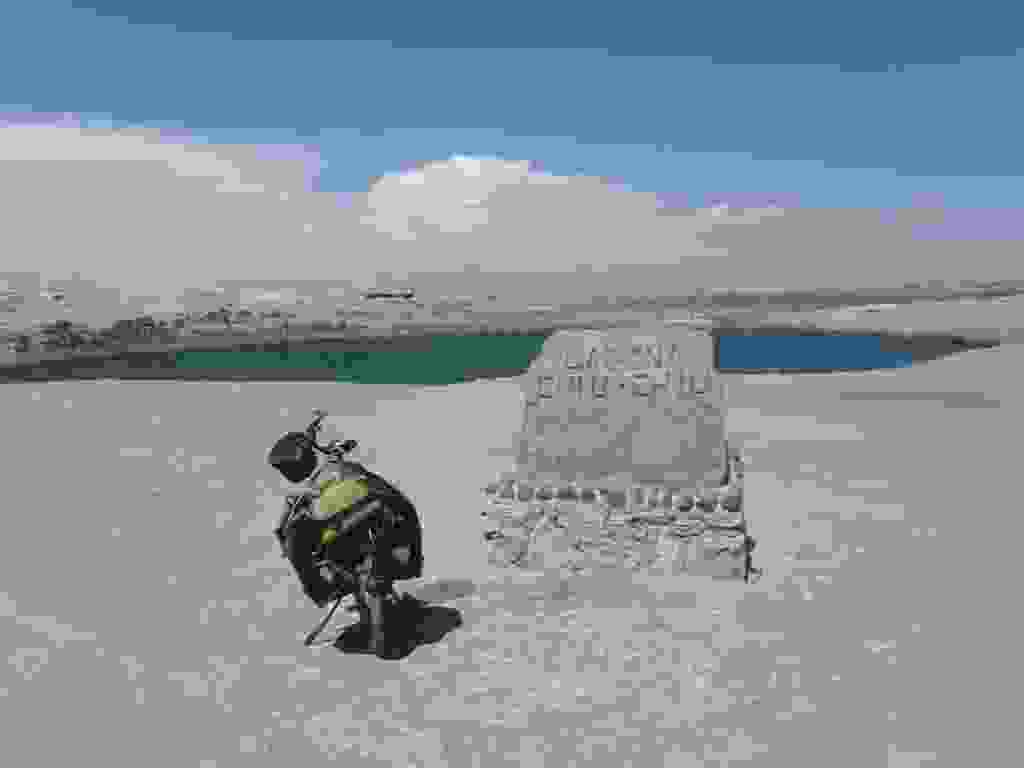
\includegraphics[width=\mywidth]{../wp-content/uploads/2015/03/P3142786-1024x768.jpg} \end{center}

Puis ça commence à monter jusqu'au premier bivouac : je ne sais pas à quelle altitude mais les effets se font un peu sentir.\\
\begin{center} 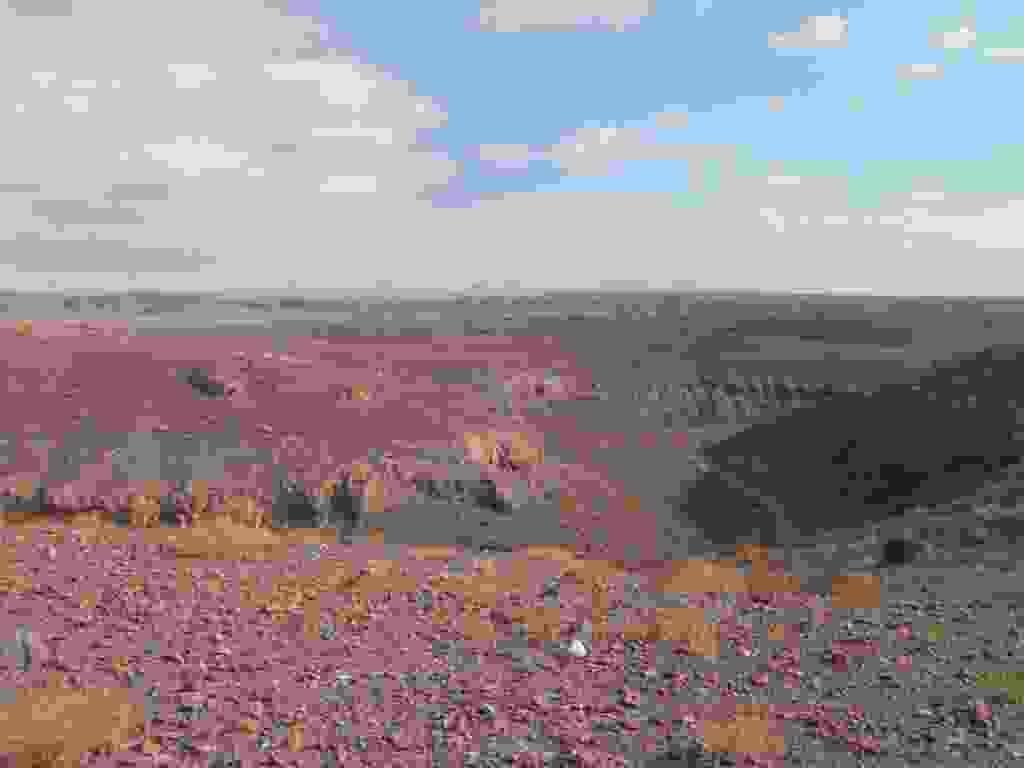
\includegraphics[width=\mywidth]{../wp-content/uploads/2015/03/P3142794-1024x768.jpg} \end{center}
\vspace{-\topsep}
\pagebreak
~
\begin{center} 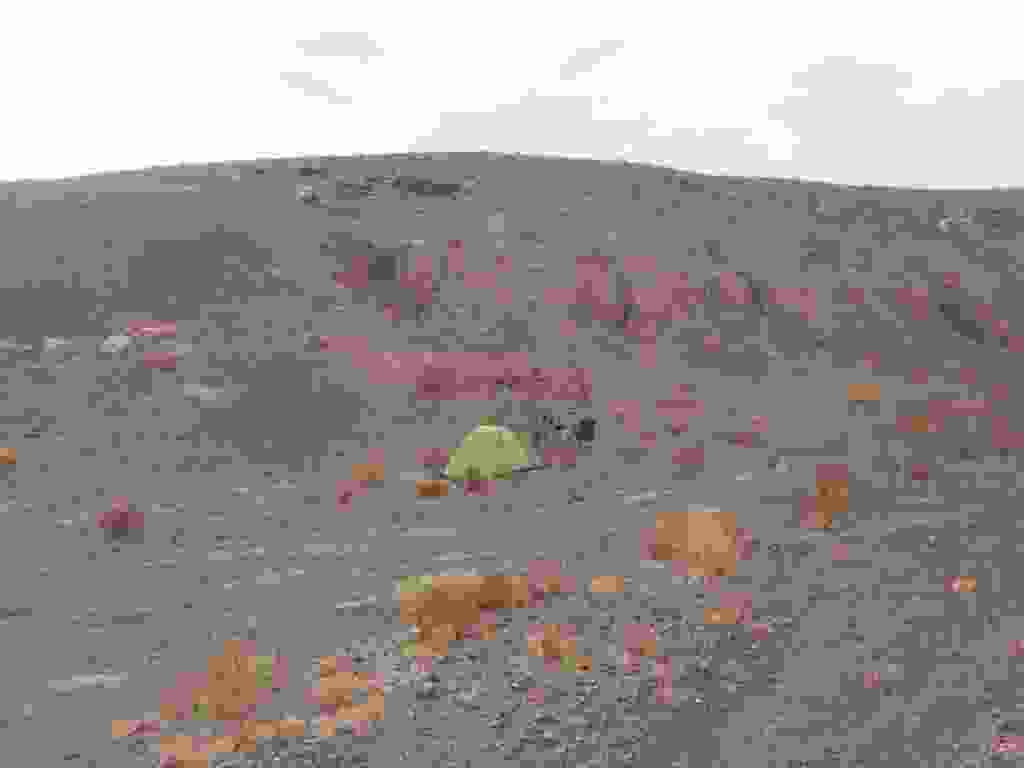
\includegraphics[width=\mywidth]{../wp-content/uploads/2015/03/P3152798-1024x768.jpg} \end{center}

 Deuxième jour, ça continue à monter sérieusement.

 Mes réserves d'eau sont un peu justes, je dois faire un aller retour de 8km vers un village pour me ravitailler. 
\begin{center} 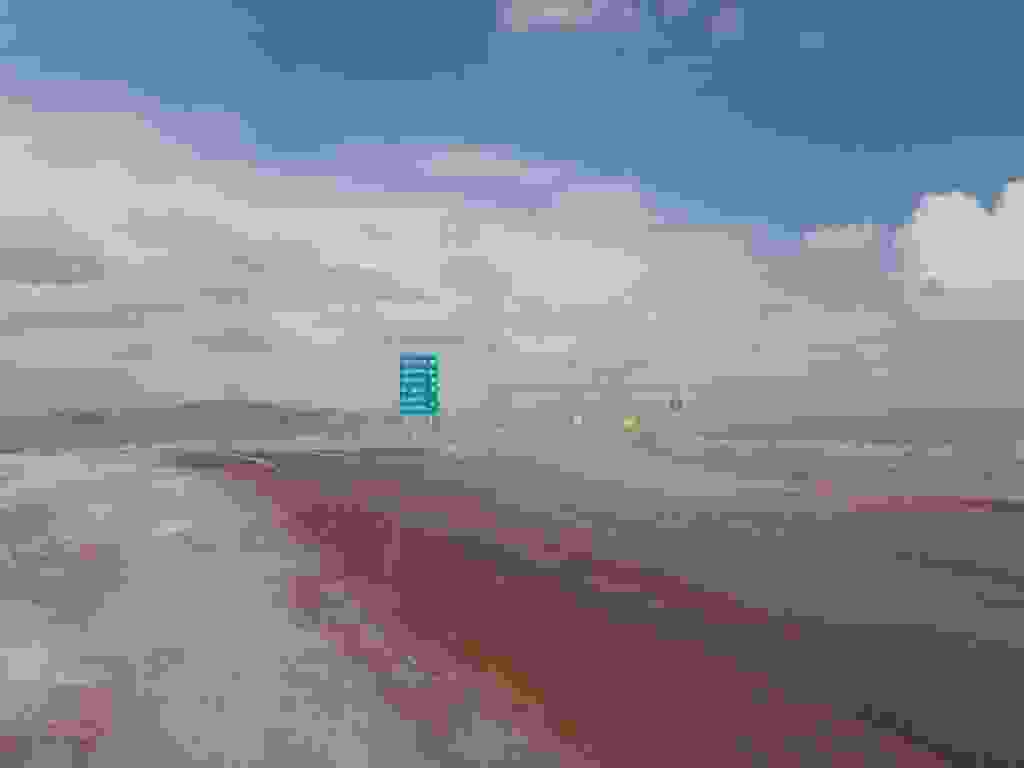
\includegraphics[width=\mywidth]{../wp-content/uploads/2015/03/P3142793-1024x768.jpg} \end{center}
\begin{center} 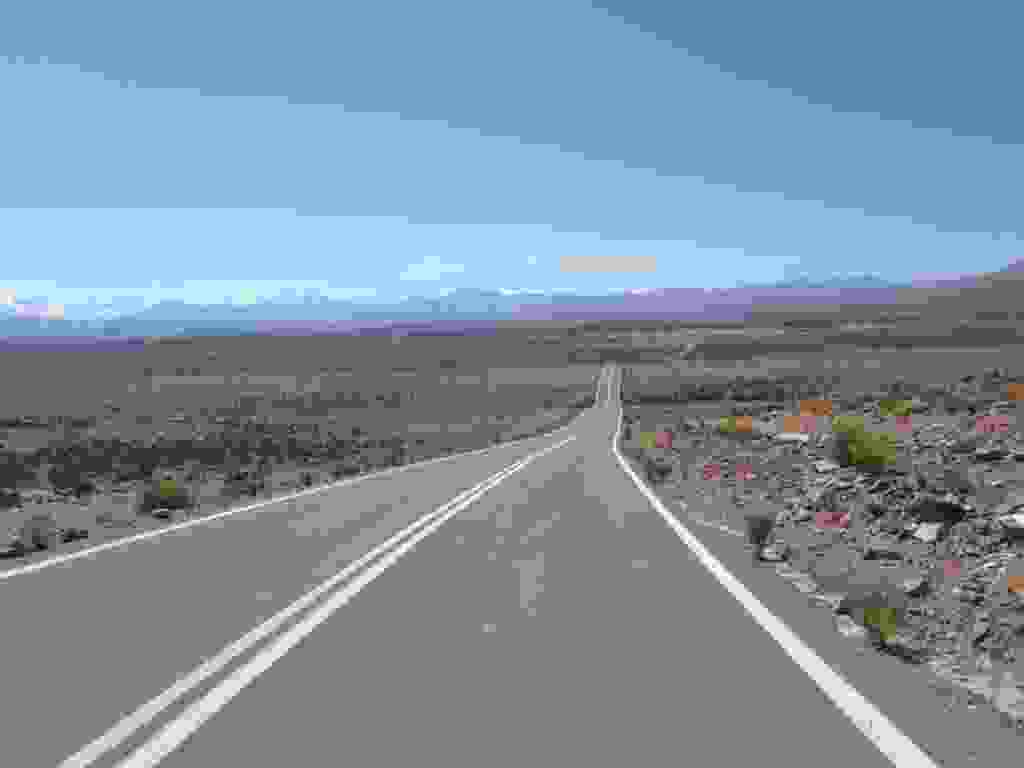
\includegraphics[width=\mywidth]{../wp-content/uploads/2015/03/P3152810-1024x768.jpg} \end{center}

 Ça valait quand même le coup, le village de Caspana est très joli.
\begin{center} 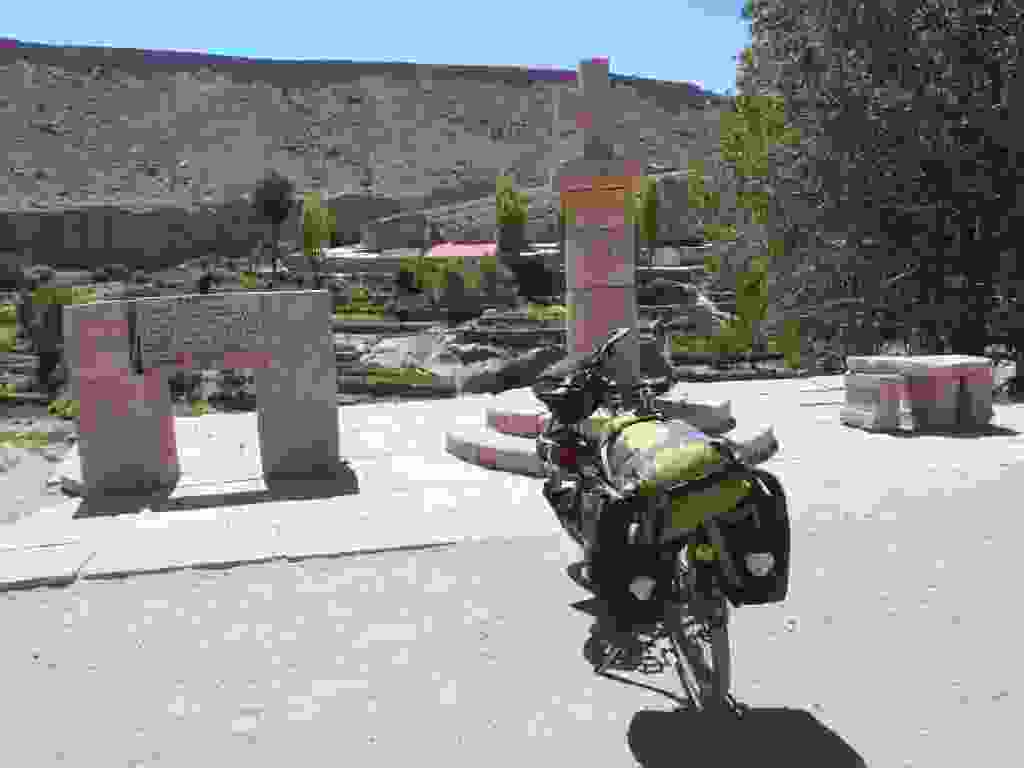
\includegraphics[width=\mywidth]{../wp-content/uploads/2015/03/P3152814-1024x768.jpg} \end{center}
\begin{center} 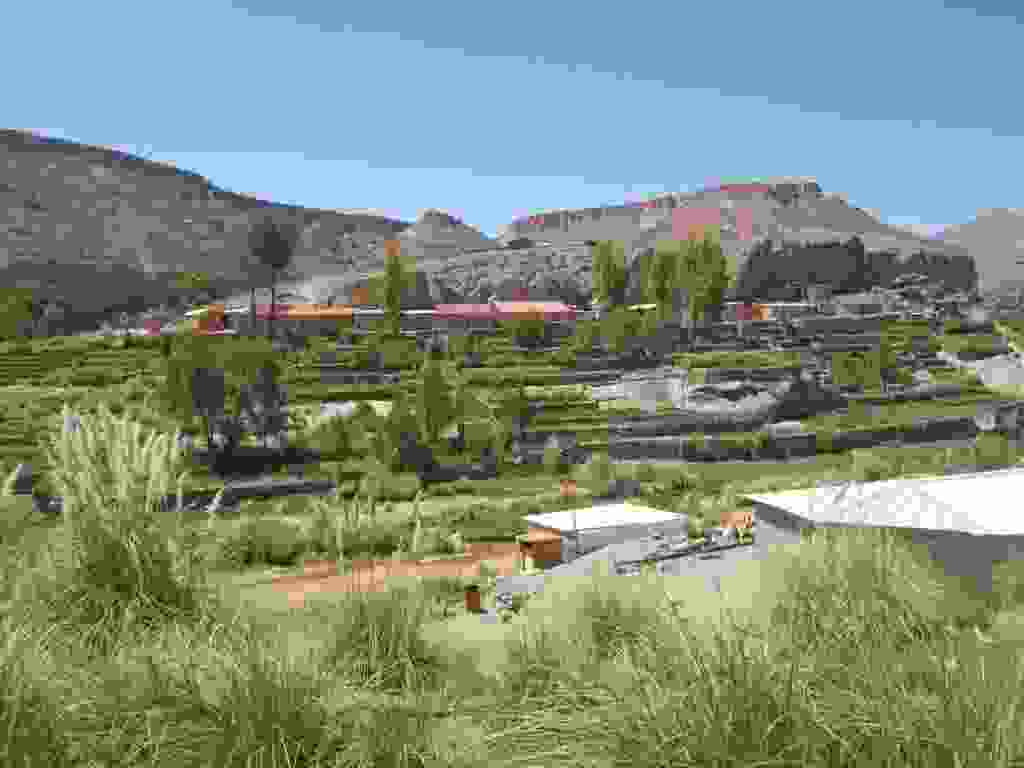
\includegraphics[width=\mywidth]{../wp-content/uploads/2015/03/P3152818-1024x768.jpg} \end{center}
\vfill
\begin{center} 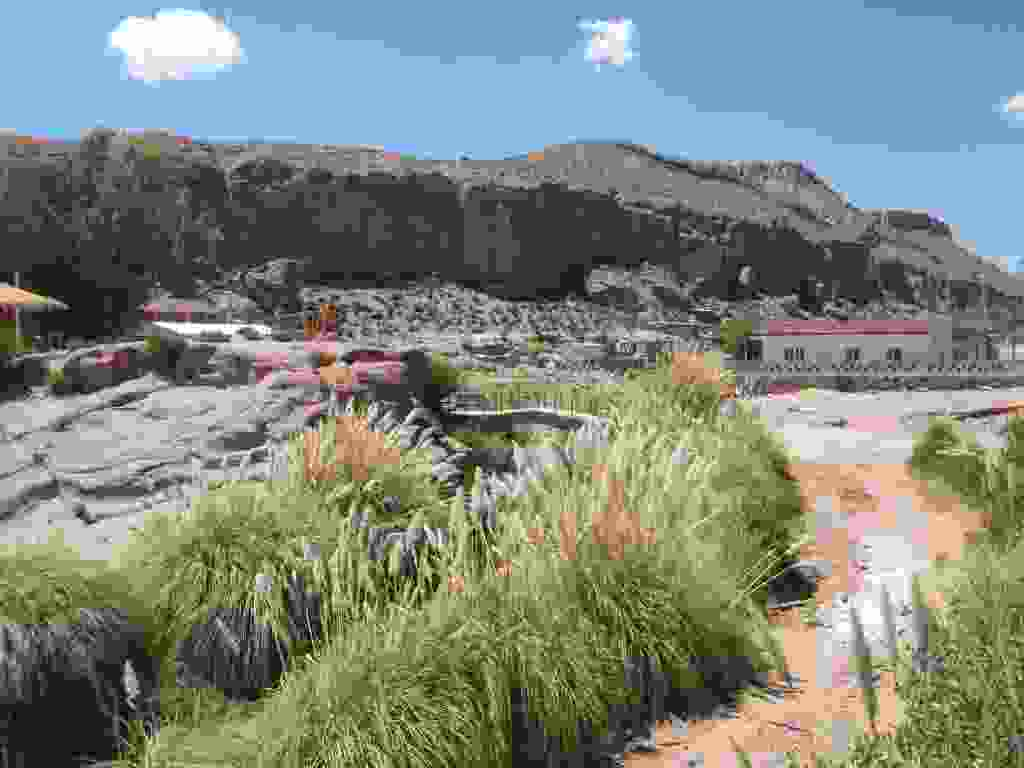
\includegraphics[width=\mywidth]{../wp-content/uploads/2015/03/P3152819-1024x768.jpg} \end{center}
\vspace{-\topsep}
\vspace{-0.75mm}

\pagebreak
~\\
\begin{center} 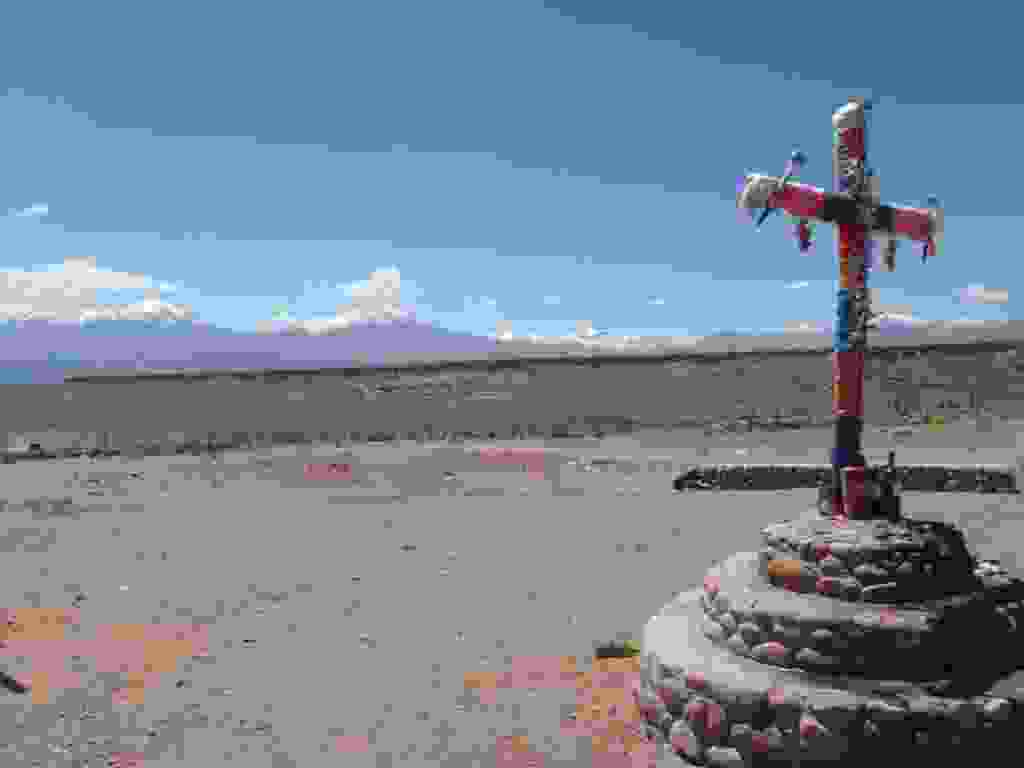
\includegraphics[width=\mywidth]{../wp-content/uploads/2015/03/P3152821-1024x768.jpg} \end{center}
\begin{center} 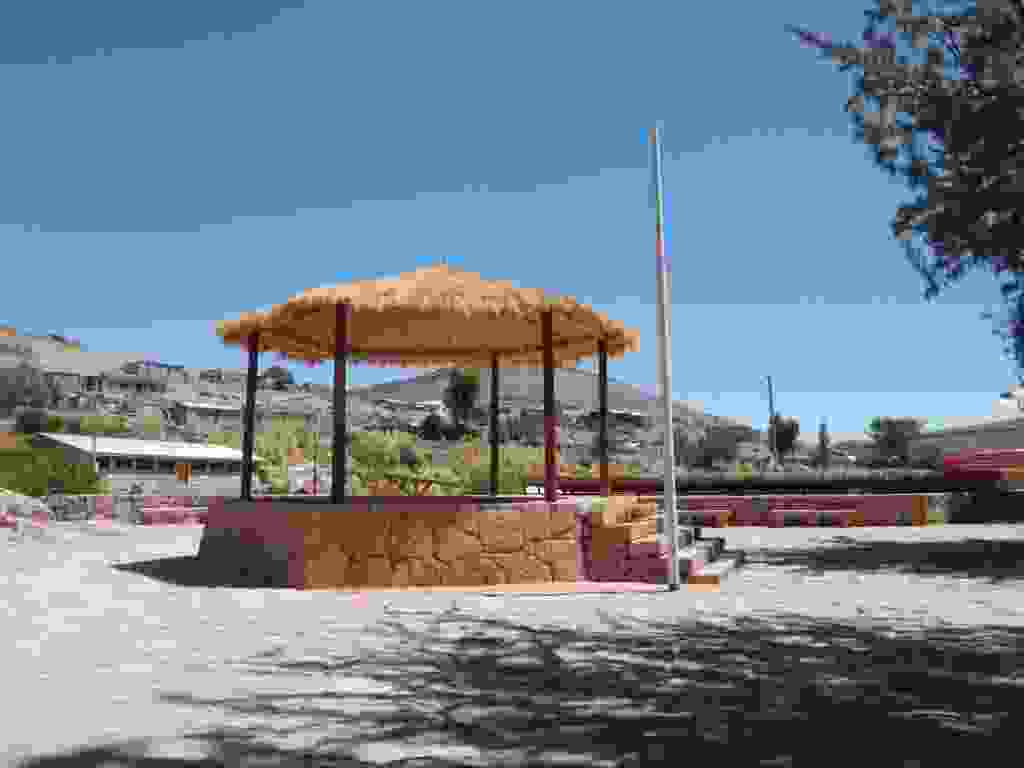
\includegraphics[width=\mywidth]{../wp-content/uploads/2015/03/P3152820-1024x768.jpg} \end{center}
\vspace{-\topsep}
\vspace{-3mm}

\pagebreak
 Je reprends la route qui continue à bien monter. Je croise quelques animaux.
\begin{center} 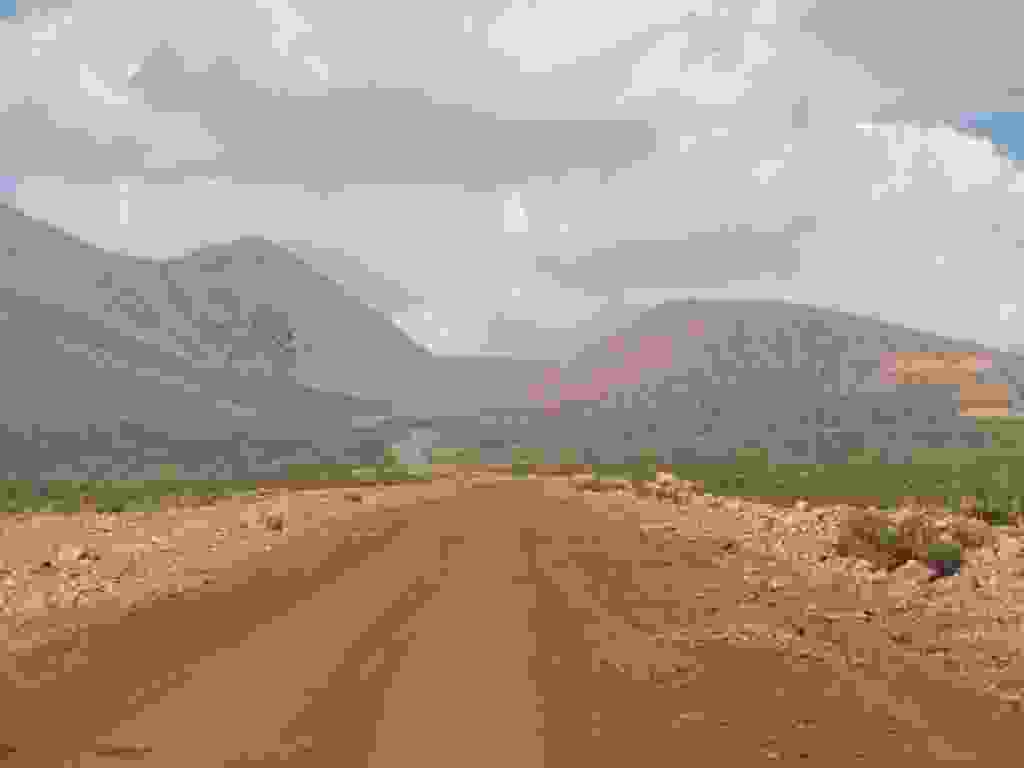
\includegraphics[width=\mywidth]{../wp-content/uploads/2015/03/P3152827-1024x768.jpg} \end{center}
\begin{center} 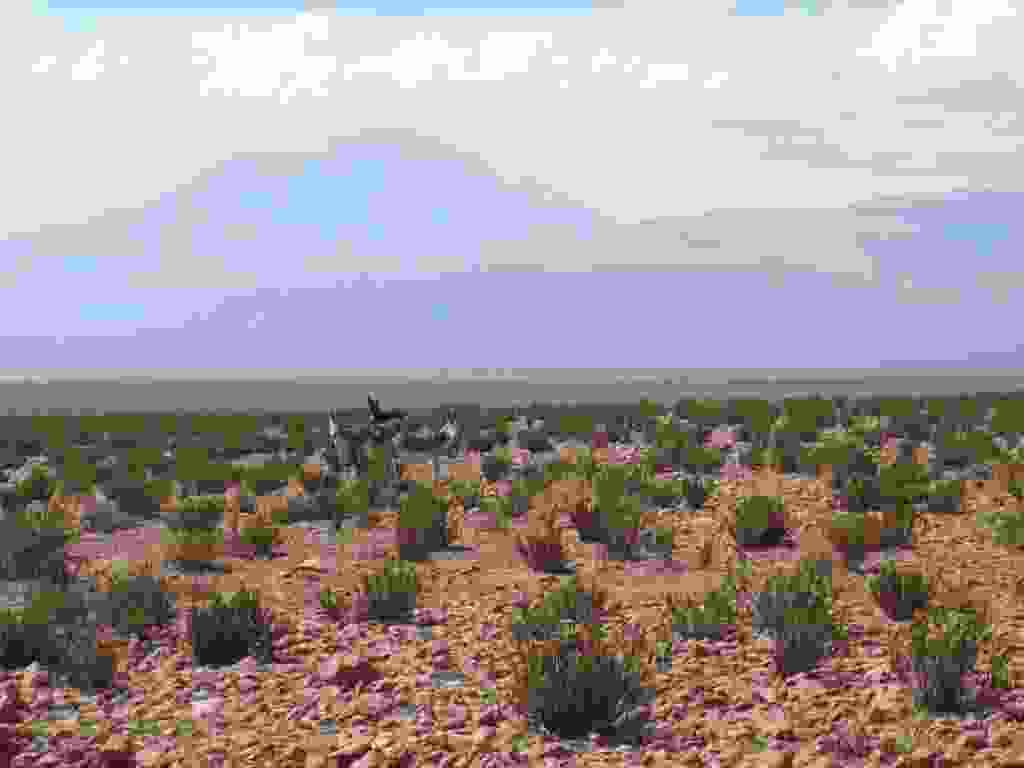
\includegraphics[width=\mywidth]{../wp-content/uploads/2015/03/P3152826-1024x768.jpg} \end{center}
\vspace{-\topsep}
\vspace{-2.75mm}
\pagebreak
~
\vspace{1mm}
\begin{center} 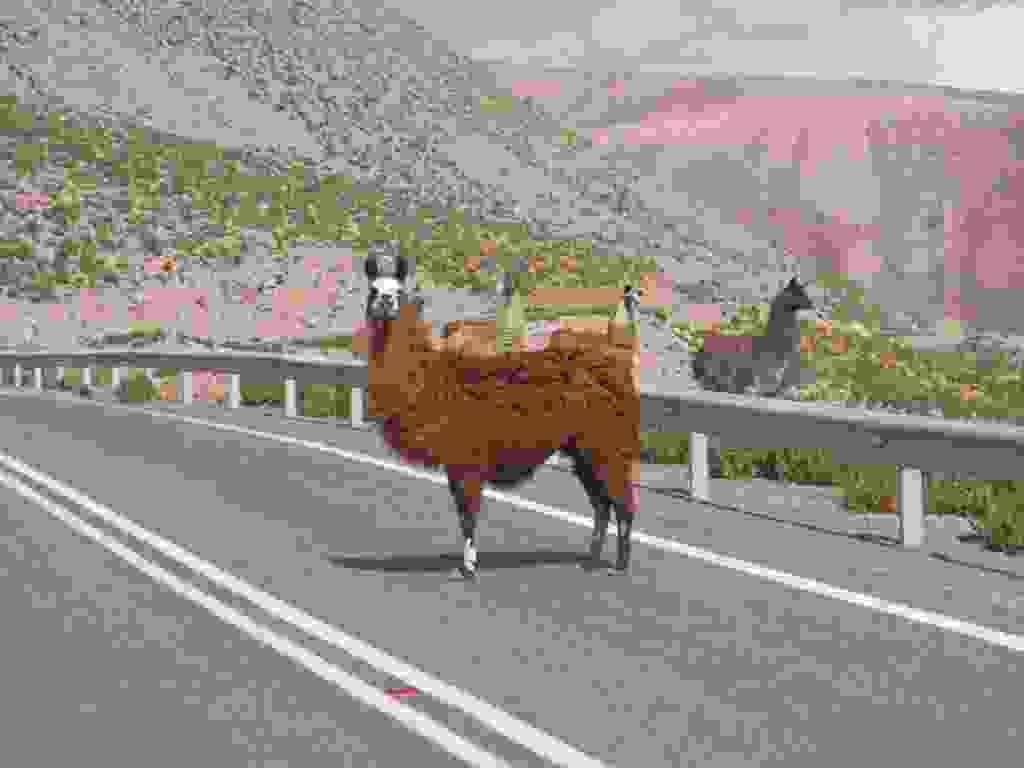
\includegraphics[width=\mywidth]{../wp-content/uploads/2015/03/P3152832-1024x768.jpg} \end{center}

 Vers 16h le temps se couvre et l´orage n´est pas loin. J´hésite à continuer mais il commence à pleuvoir, je me dépêche de poser la tente où je peux.
\begin{center} 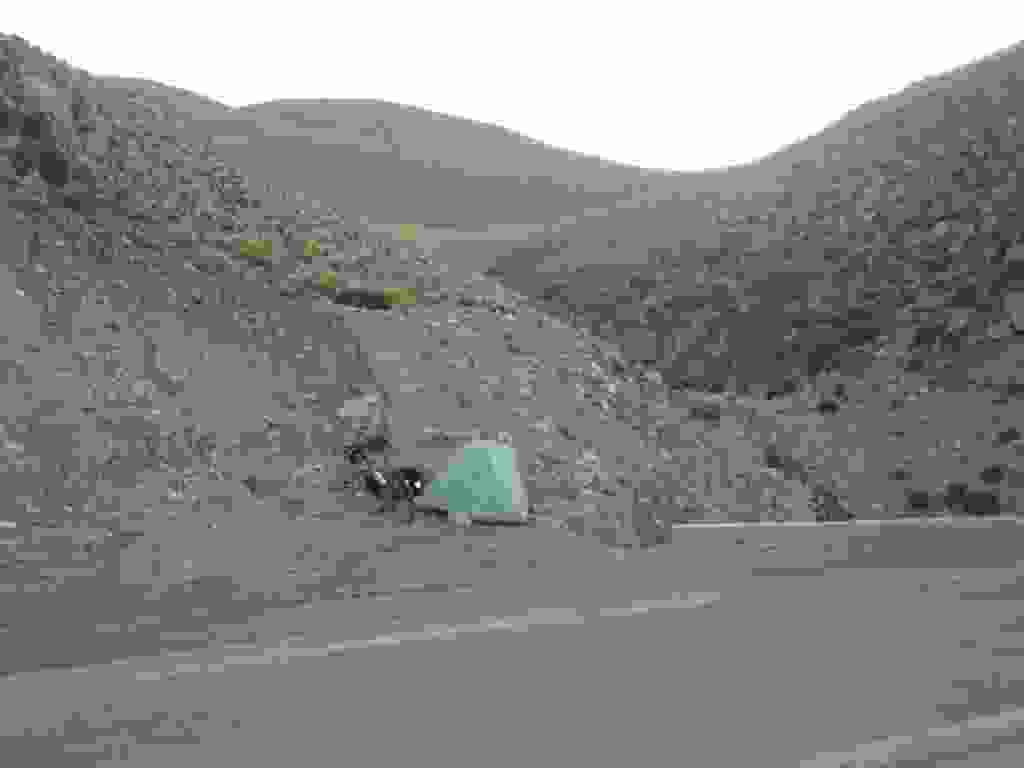
\includegraphics[width=\mywidth]{../wp-content/uploads/2015/03/P3162833-1024x768.jpg} \end{center}
\vspace{-\topsep}

\pagebreak
 Le 3\ieme\ jour débute sous un beau ciel bleu et des paysages magnifiques. 
\begin{center} 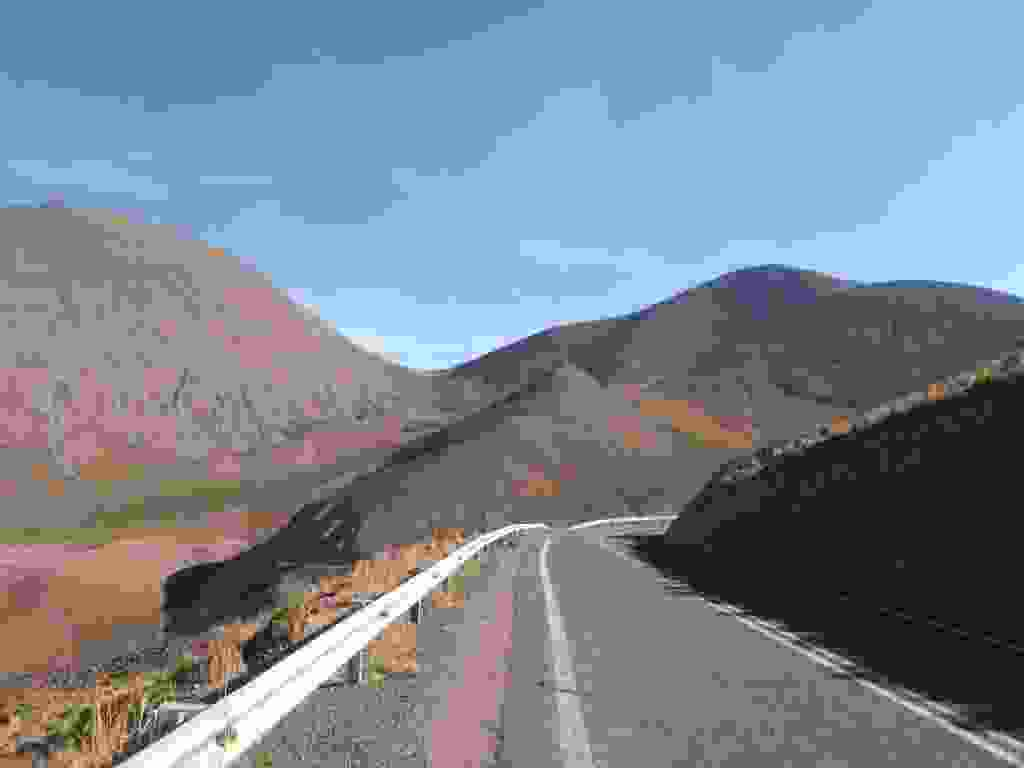
\includegraphics[width=\mywidth]{../wp-content/uploads/2015/03/P3162835-1024x768.jpg} \end{center}
~\\
\begin{center} 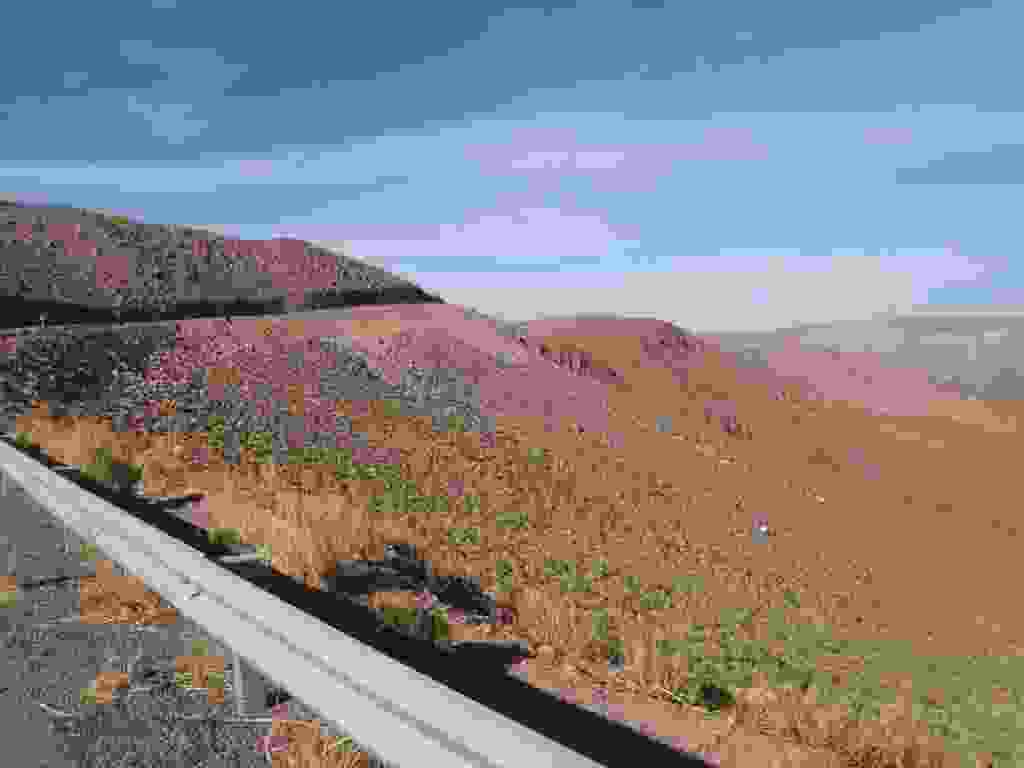
\includegraphics[width=\mywidth]{../wp-content/uploads/2015/03/P3162836-1024x768.jpg} \end{center}
\begin{center} 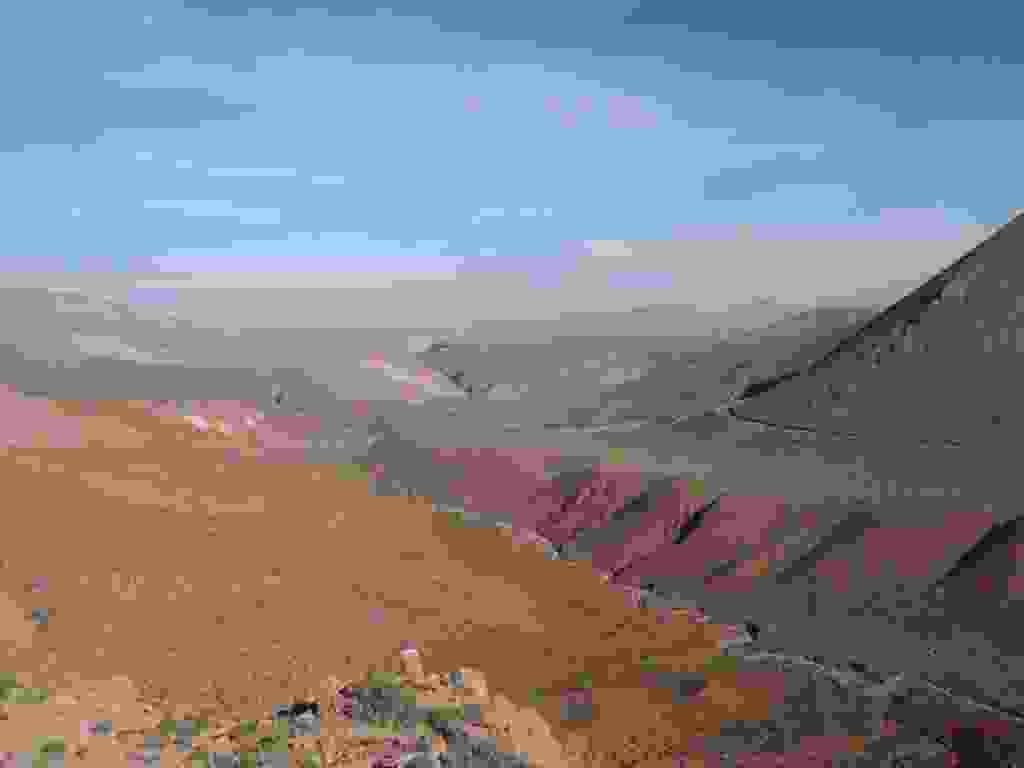
\includegraphics[width=\mywidth]{../wp-content/uploads/2015/03/P3162837-1024x768.jpg} \end{center}
\begin{center} 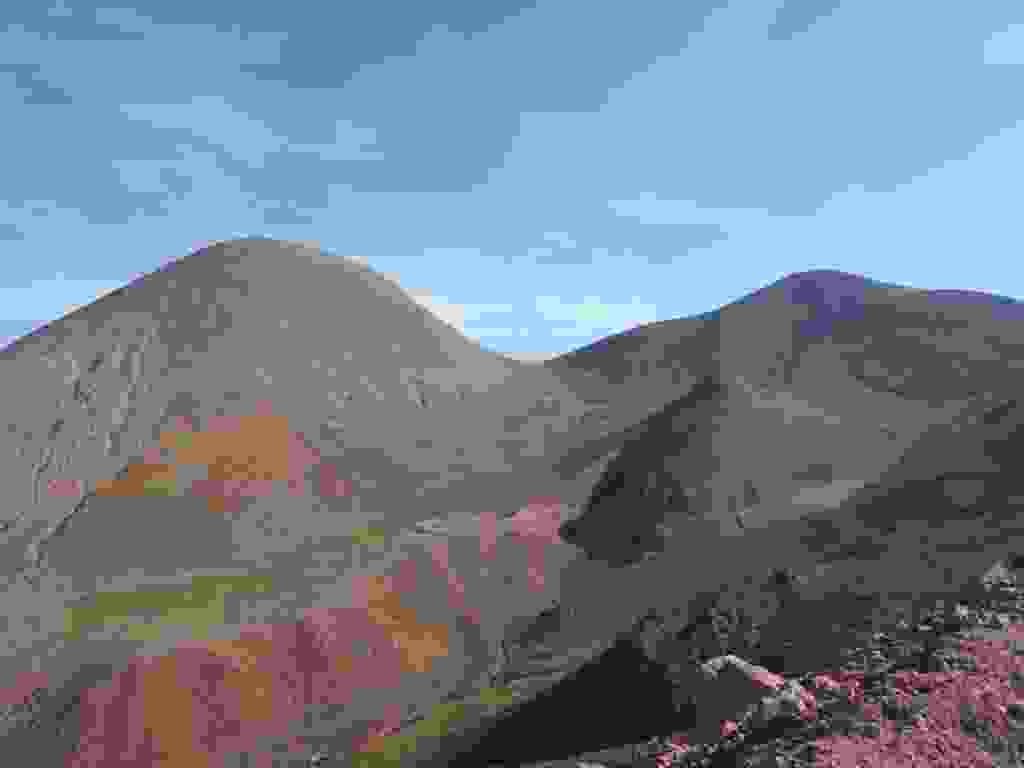
\includegraphics[width=\mywidth]{../wp-content/uploads/2015/03/P31628401-1024x768.jpg} \end{center}
\begin{center} 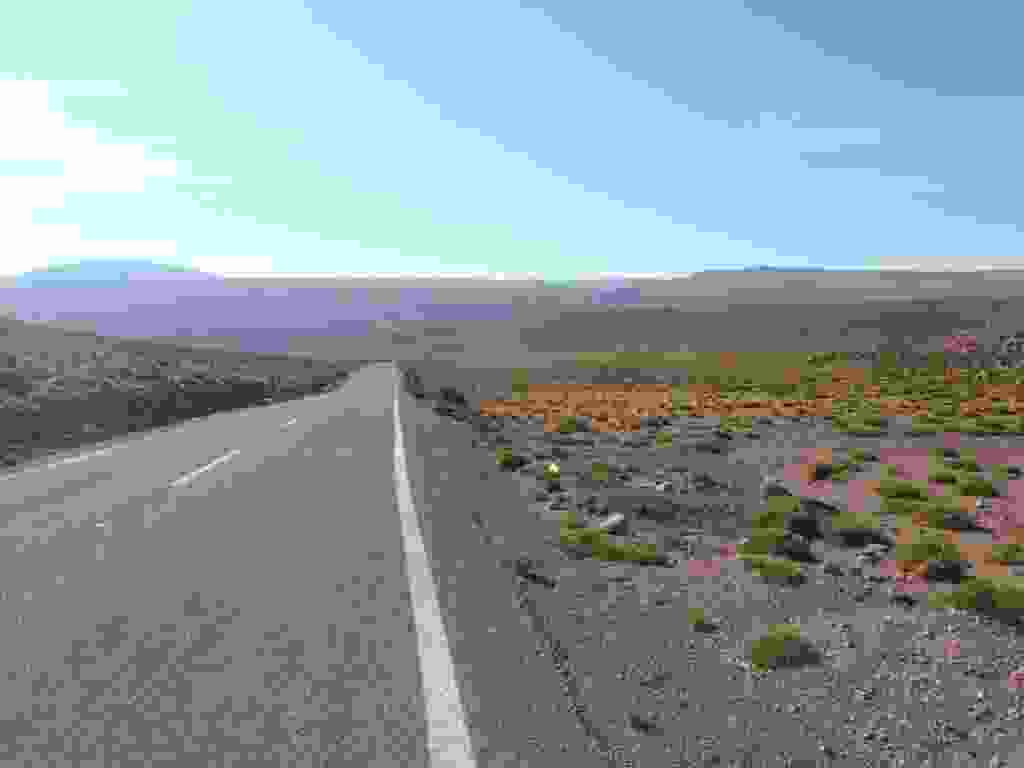
\includegraphics[width=\mywidth]{../wp-content/uploads/2015/03/P31628411-1024x768.jpg} \end{center}
\vfill
\begin{center} 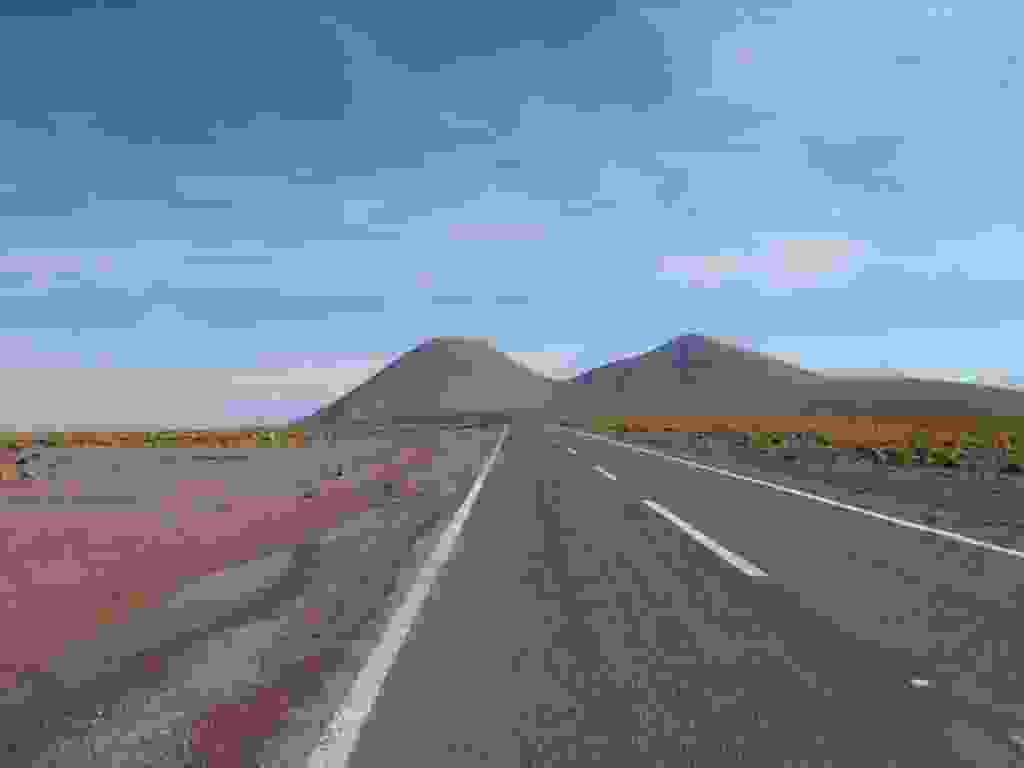
\includegraphics[width=\mywidth]{../wp-content/uploads/2015/03/P31628441-1024x768.jpg} \end{center}
\vspace{-\topsep}
\vspace{-0.75mm}

\pagebreak
~\\
\begin{center} 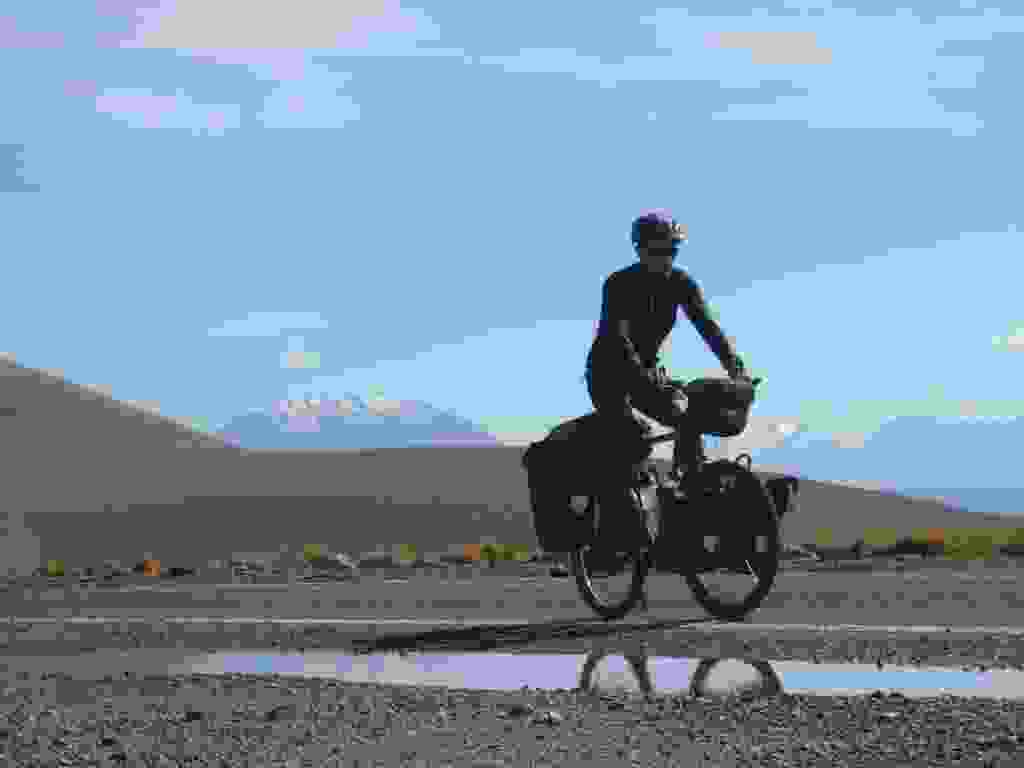
\includegraphics[width=\mywidth]{../wp-content/uploads/2015/03/P3162848-1024x768.jpg} \end{center}
\begin{center} 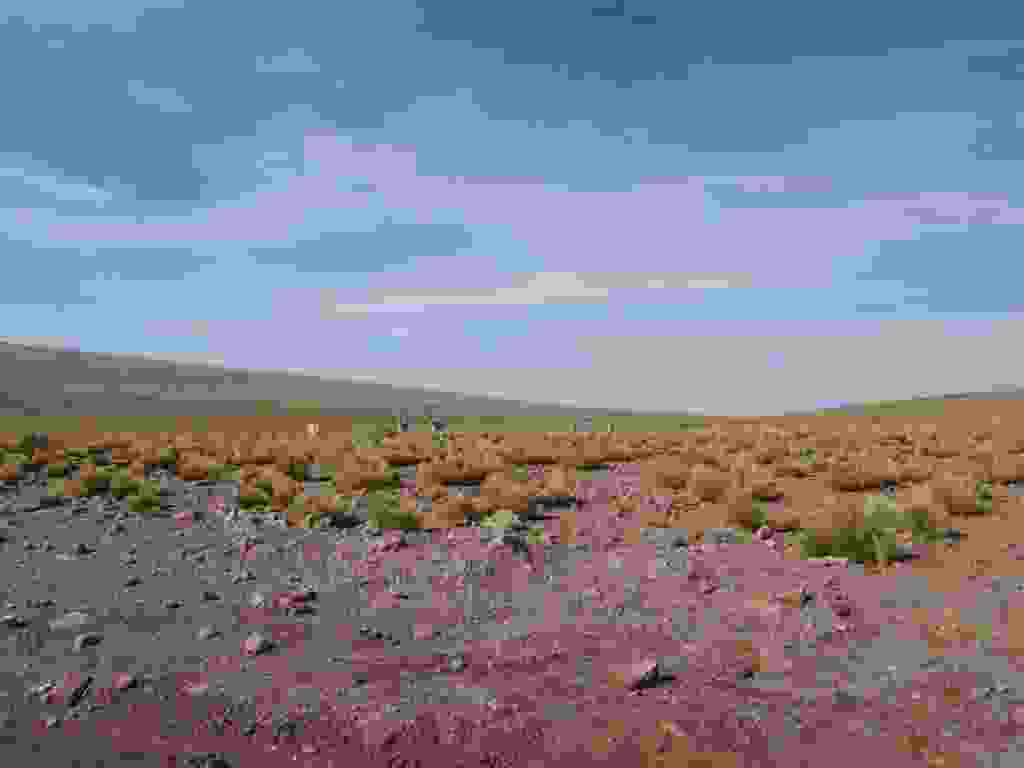
\includegraphics[width=\mywidth]{../wp-content/uploads/2015/03/P31628491-1024x768.jpg} \end{center}

~\\

\pagebreak
Mais encore une fois ça se couvre dès midi et je roule pour essayer d'atteindre les geysers rapidement. 
\begin{center} 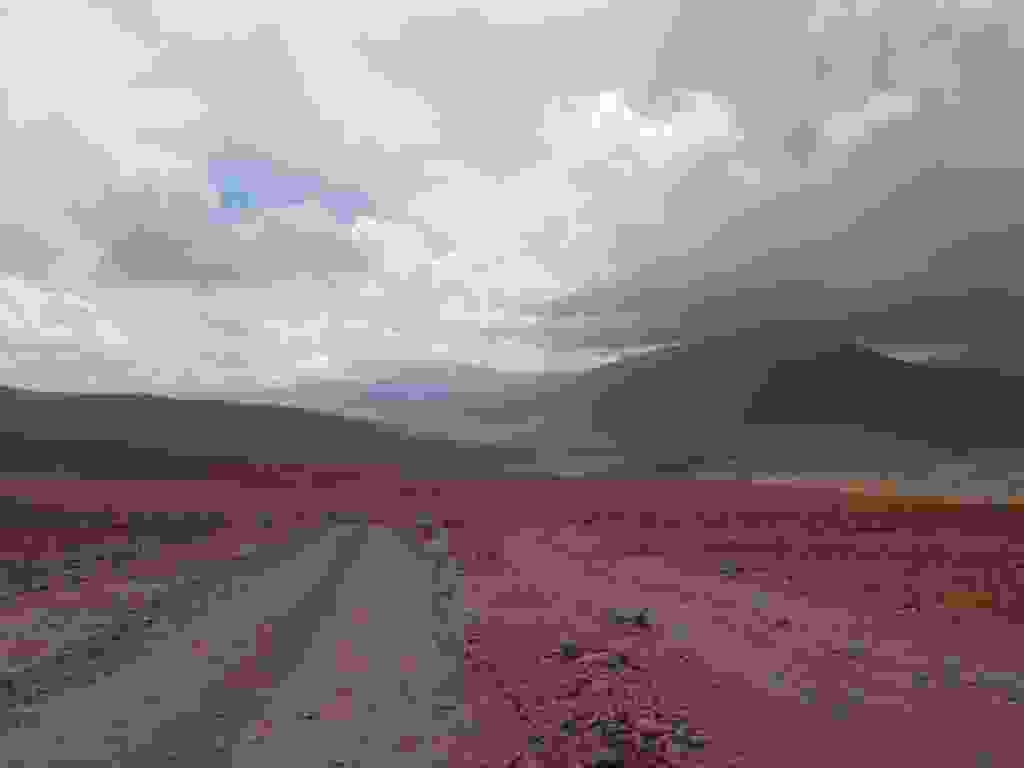
\includegraphics[width=\mywidth]{../wp-content/uploads/2015/03/P3162854-1024x768.jpg} \end{center}
\begin{center} 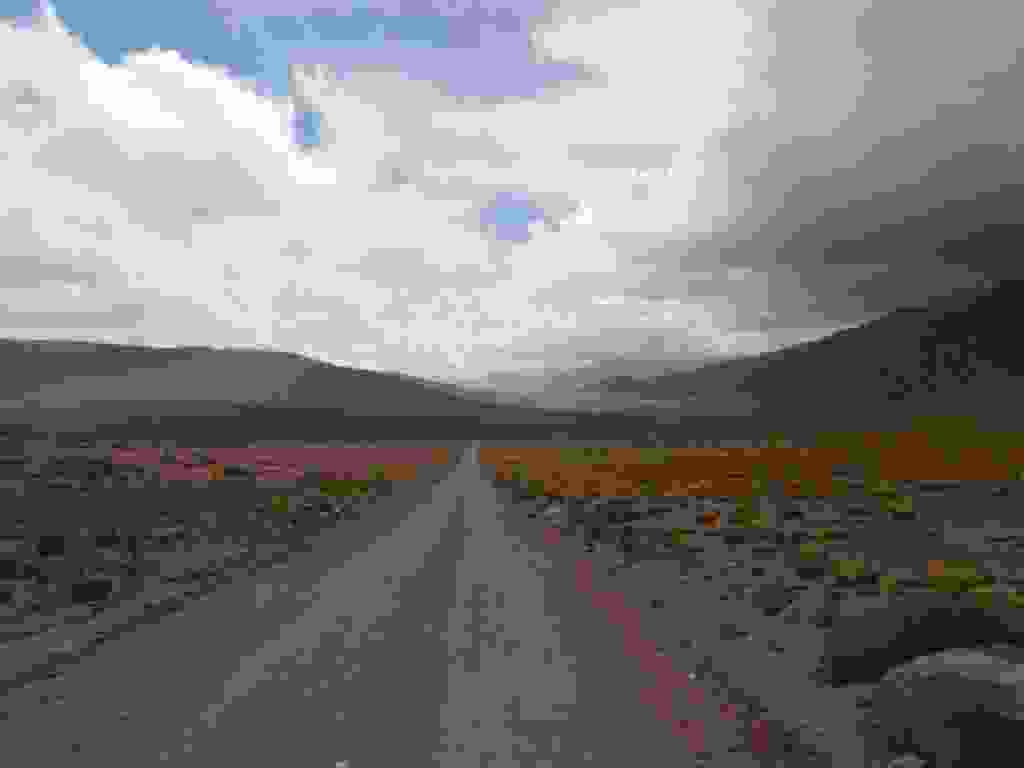
\includegraphics[width=\mywidth]{../wp-content/uploads/2015/03/P3162856-1024x768.jpg} \end{center}

 Par chance la fin n'est pas trop difficile et j'arrive assez rapidement au refuge d'El Tatio à 4200m. 

\pagebreak
 Les gardiens sont un peu surpris de voir arriver un vélo, surtout que les touristes ne viennent que le matin et dès 11h il n'y a plus personne. 
\begin{center} 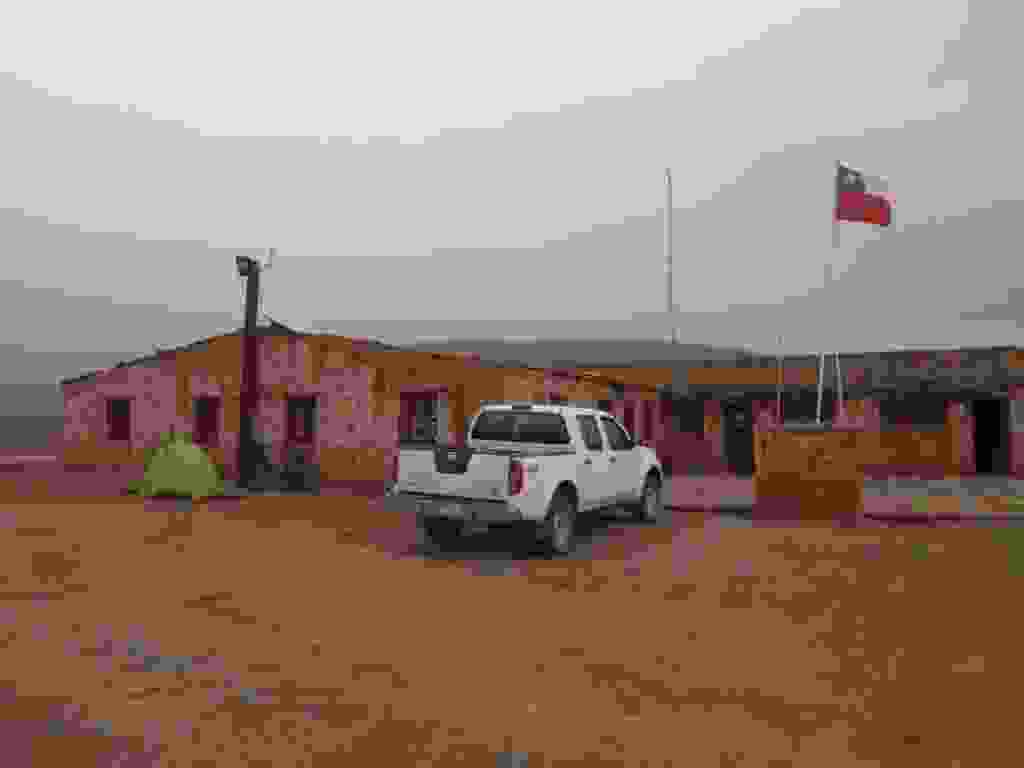
\includegraphics[width=\mywidth]{../wp-content/uploads/2015/03/P3162862-1024x768.jpg} \end{center}

 J'ai le champ de geysers pour moi tout seul l'après midi. 
\begin{center} 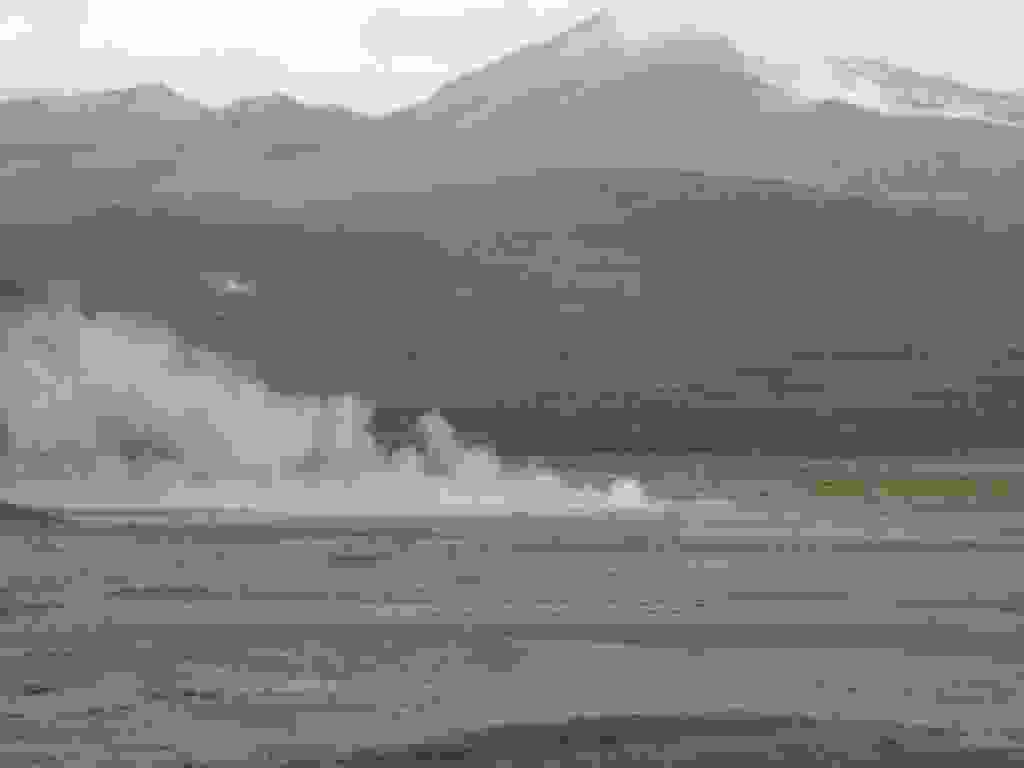
\includegraphics[width=\mywidth]{../wp-content/uploads/2015/03/P3162868-1024x768.jpg} \end{center}
\vspace{-\topsep}

\pagebreak
~\\
\begin{center} 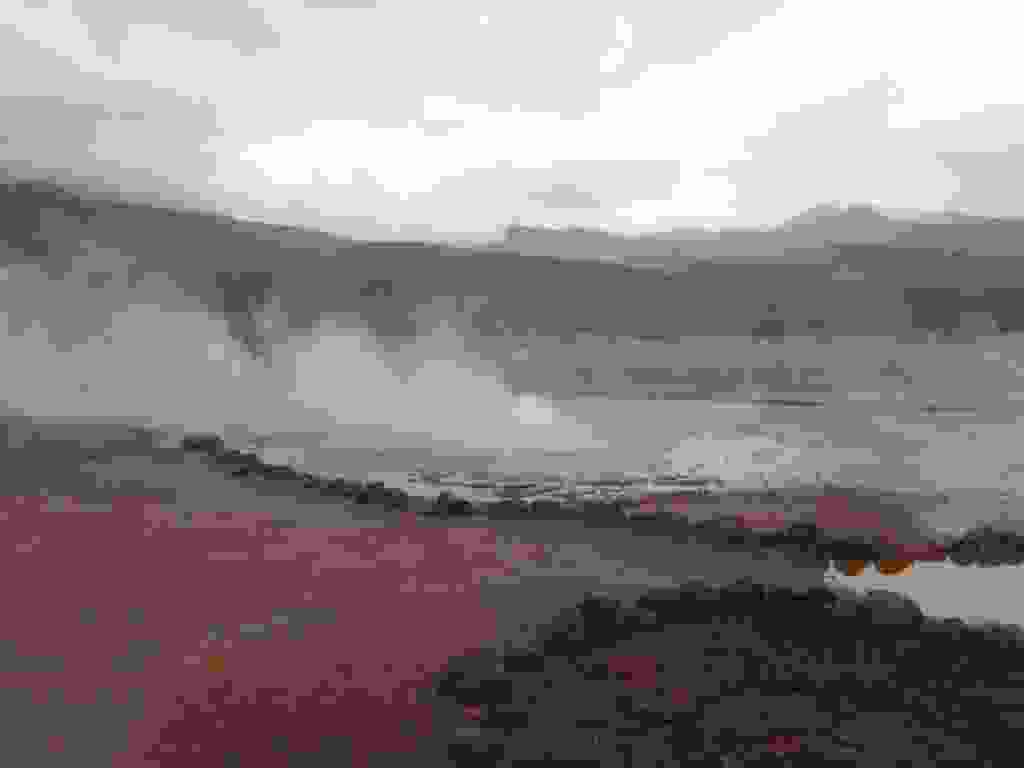
\includegraphics[width=\mywidth]{../wp-content/uploads/2015/03/P3162874-1024x768.jpg} \end{center}
~
\begin{center} 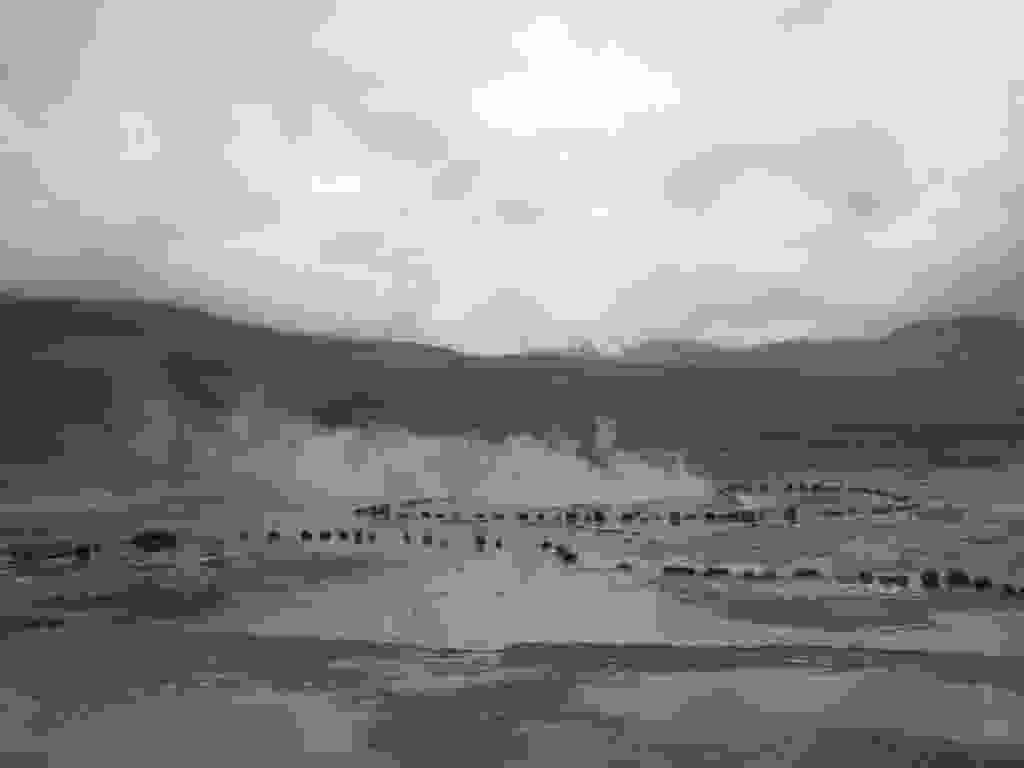
\includegraphics[width=\mywidth]{../wp-content/uploads/2015/03/P3162878-1024x768.jpg} \end{center}
\begin{center} 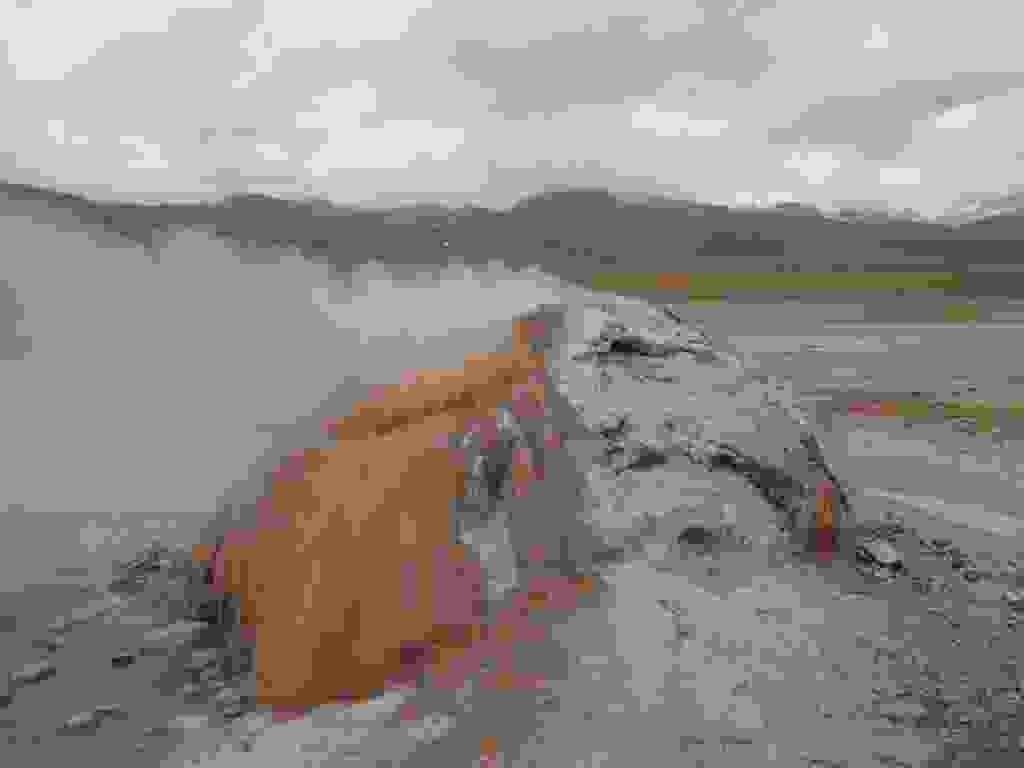
\includegraphics[width=\mywidth]{../wp-content/uploads/2015/03/P3162879-1024x768.jpg} \end{center}
\begin{center} 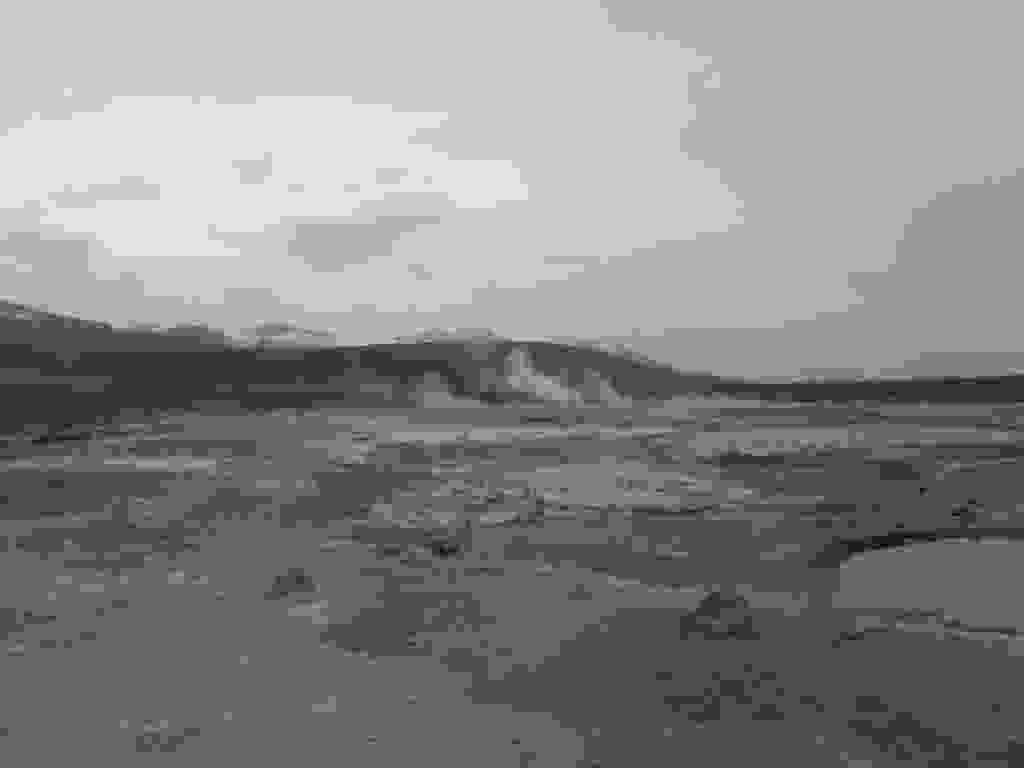
\includegraphics[width=\mywidth]{../wp-content/uploads/2015/03/P3162885-1024x768.jpg} \end{center}
\begin{center} 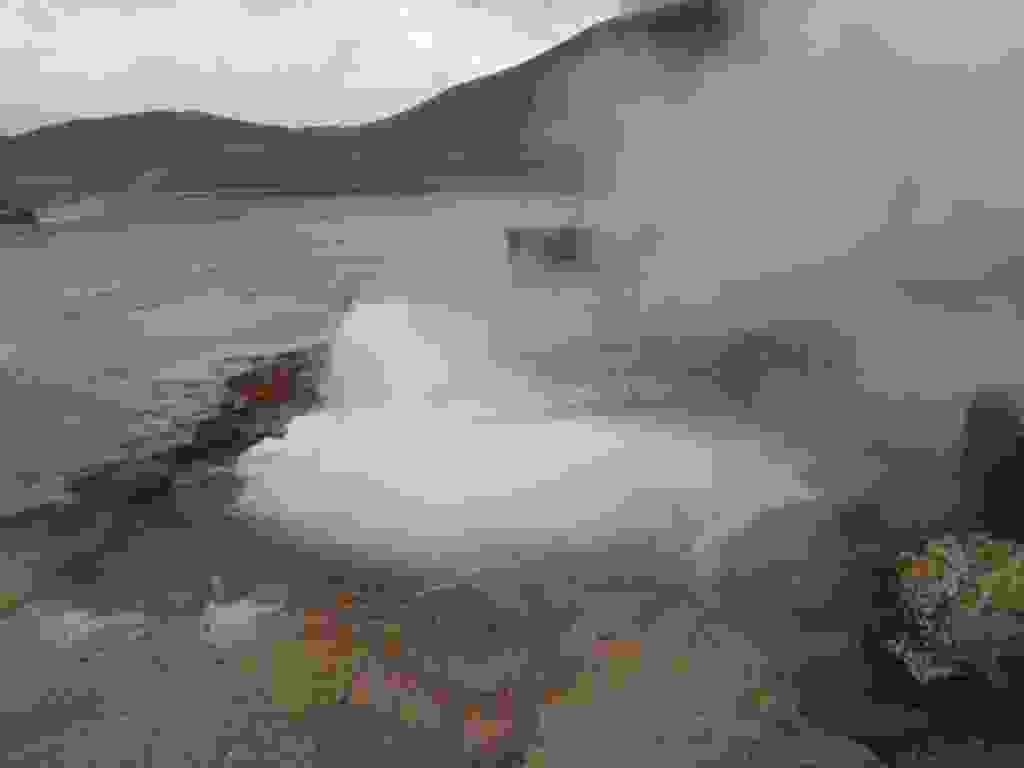
\includegraphics[width=\mywidth]{../wp-content/uploads/2015/03/P3162886-1024x768.jpg} \end{center}
\vfill
\begin{center} 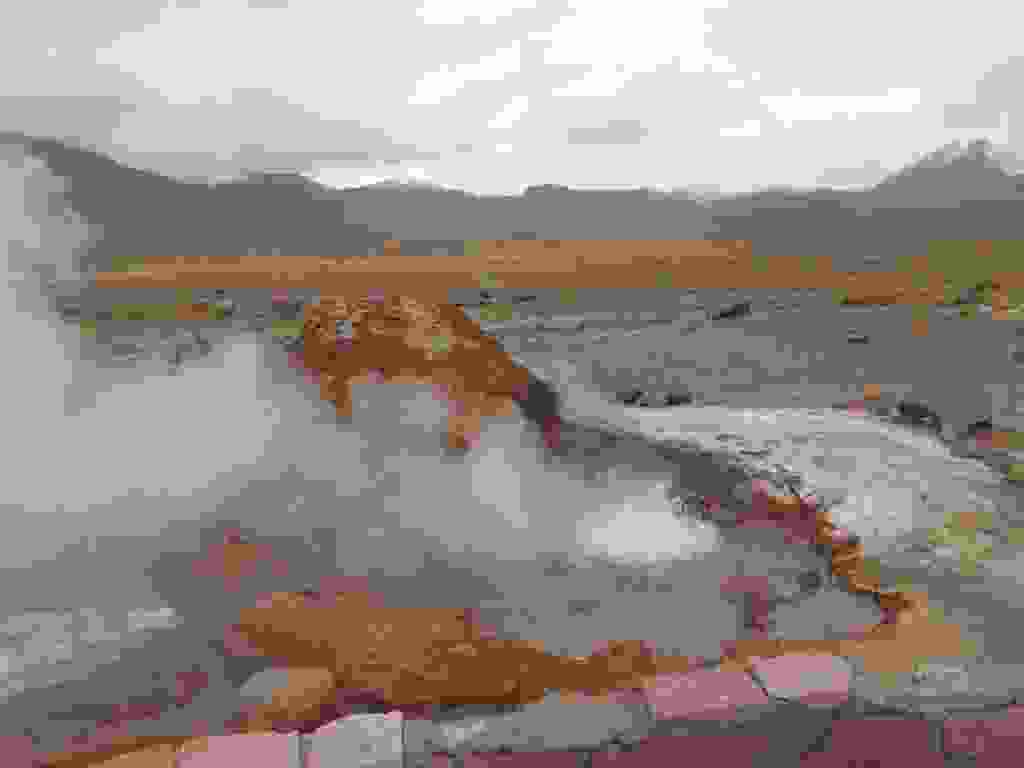
\includegraphics[width=\mywidth]{../wp-content/uploads/2015/03/P3162890-1024x768.jpg} \end{center}
\vspace{-\topsep}
\vspace{-0.75mm}
\pagebreak
~\\
\vspace{1mm}
\begin{center} 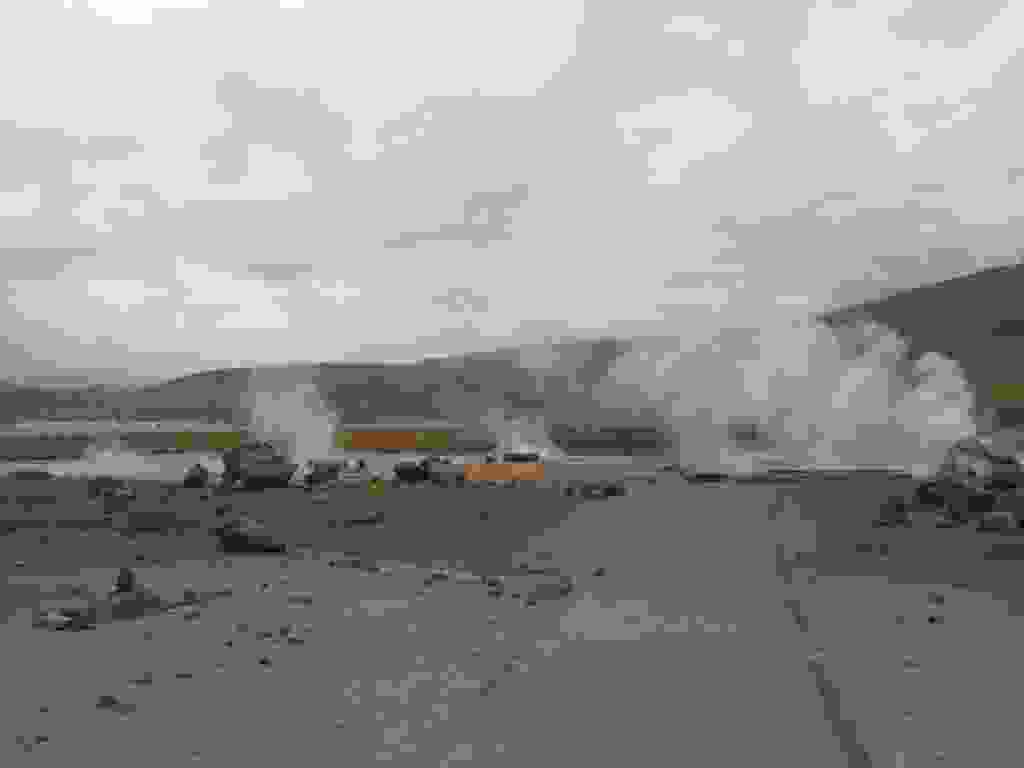
\includegraphics[width=\mywidth]{../wp-content/uploads/2015/03/P3162892-1024x768.jpg} \end{center}

 Ainsi que la piscine d'eau chaude ! 
\begin{center} 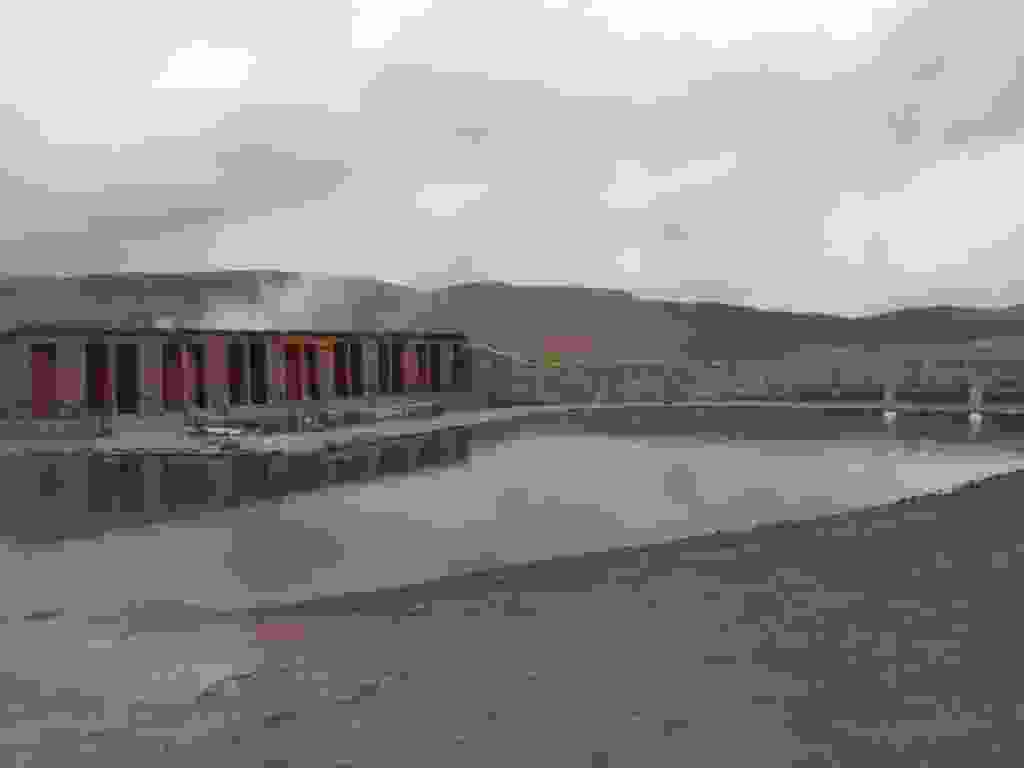
\includegraphics[width=\mywidth]{../wp-content/uploads/2015/03/P3162884-1024x768.jpg} \end{center}
\vspace{-\topsep}

\pagebreak
  Le lendemain matin un petit tour aux geysers, la lumière est différente mais il y a monde cette fois. 
\begin{center} 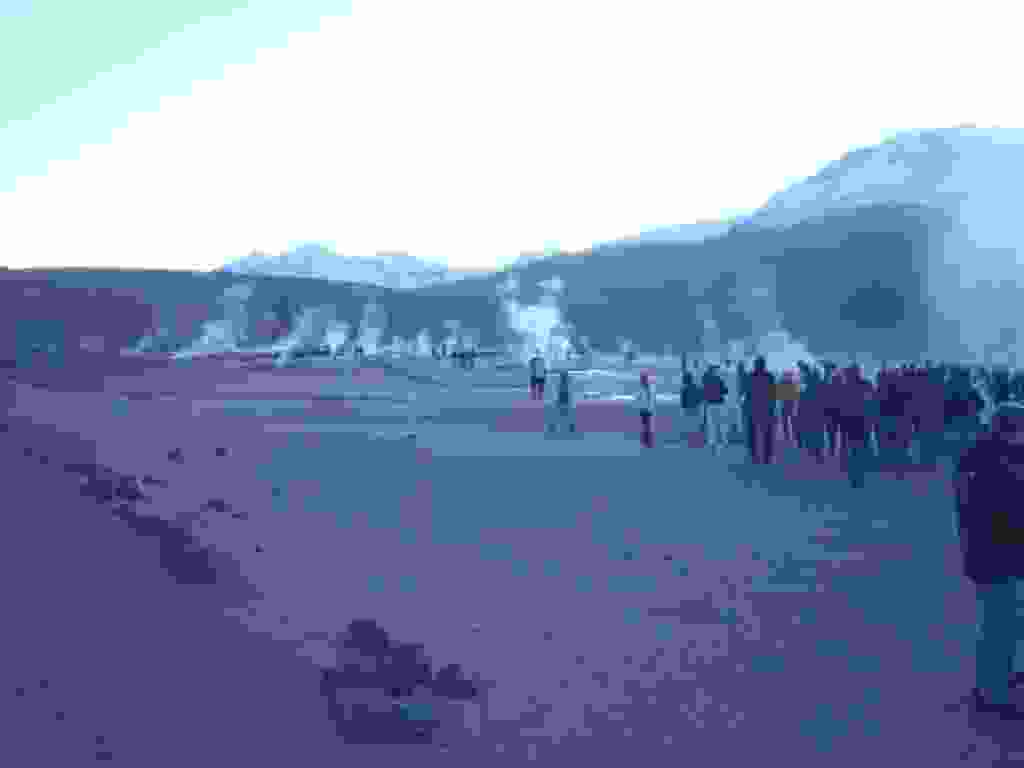
\includegraphics[width=\mywidth]{../wp-content/uploads/2015/03/P3172894-1024x768.jpg} \end{center}
~
\begin{center} 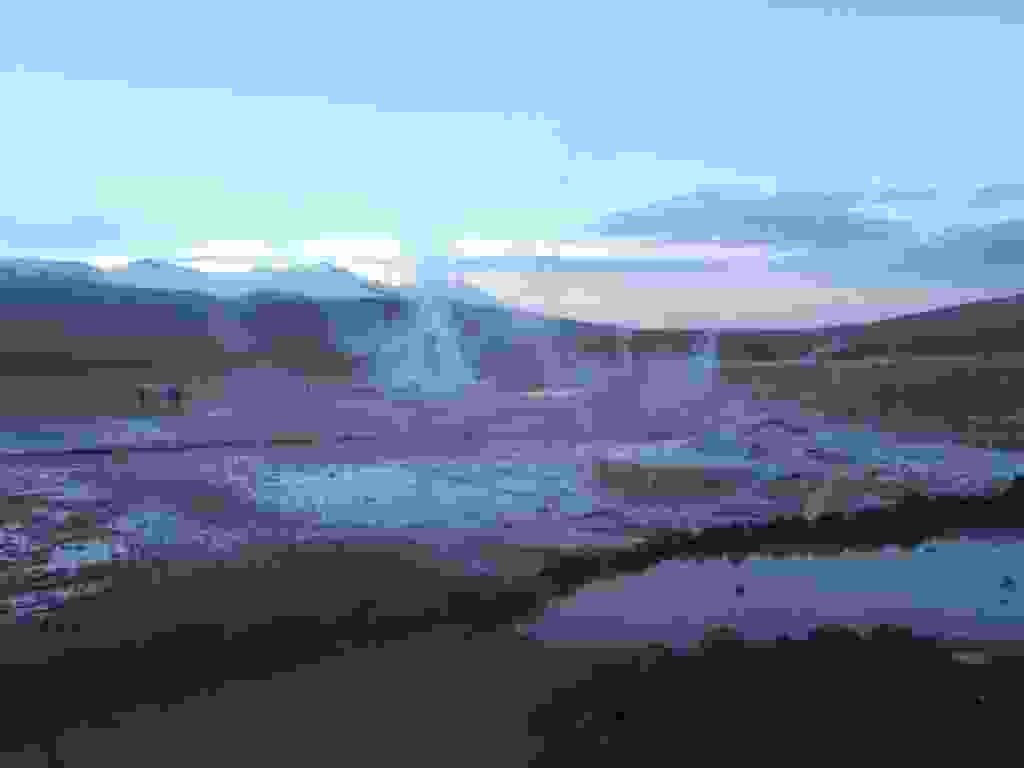
\includegraphics[width=\mywidth]{../wp-content/uploads/2015/03/P3172897-1024x768.jpg} \end{center}
\begin{center} 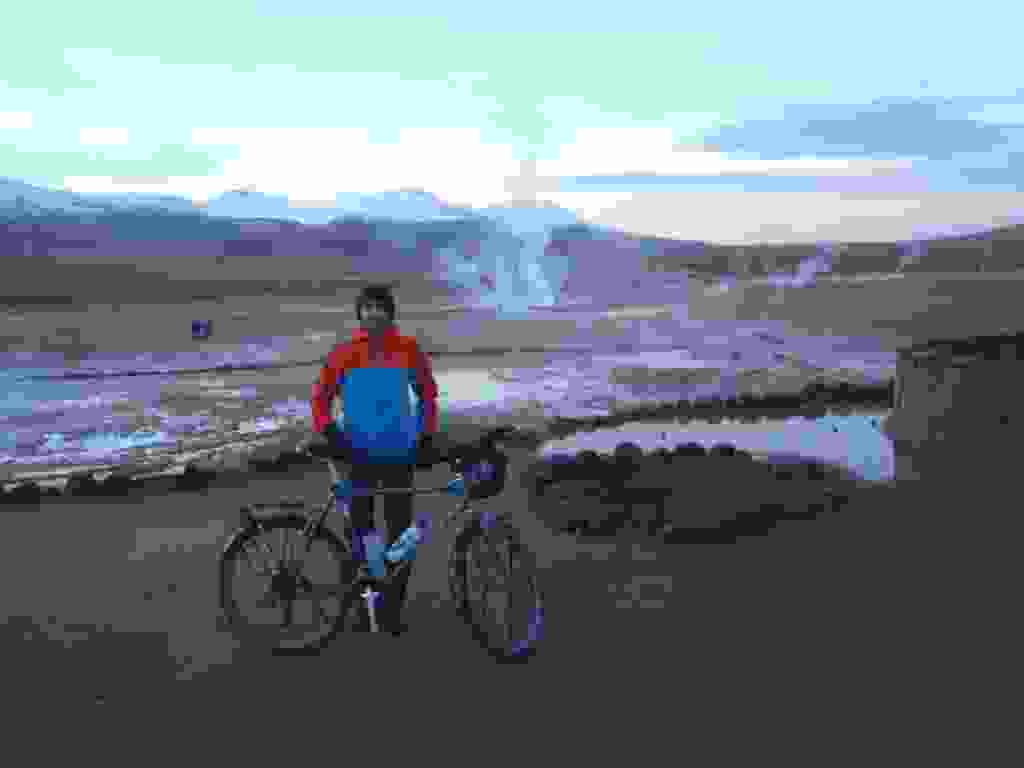
\includegraphics[width=\mywidth]{../wp-content/uploads/2015/03/P3172898-1024x768.jpg} \end{center}
\begin{center} 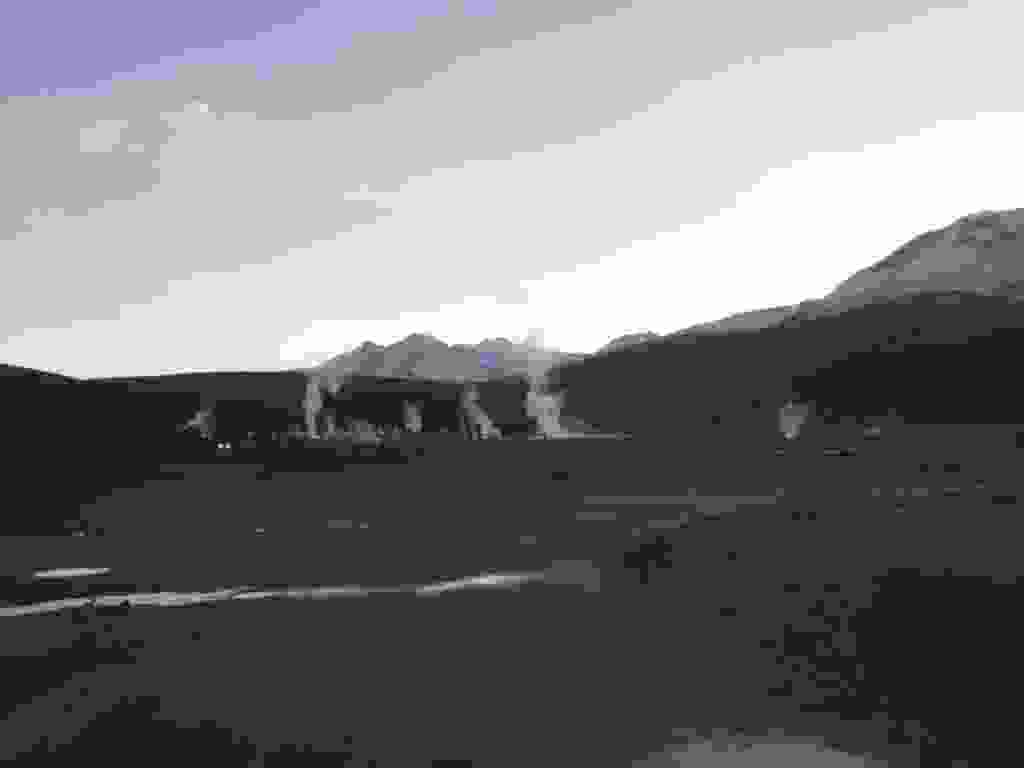
\includegraphics[width=\mywidth]{../wp-content/uploads/2015/03/P3172900-1024x768.jpg} \end{center}
\begin{center} 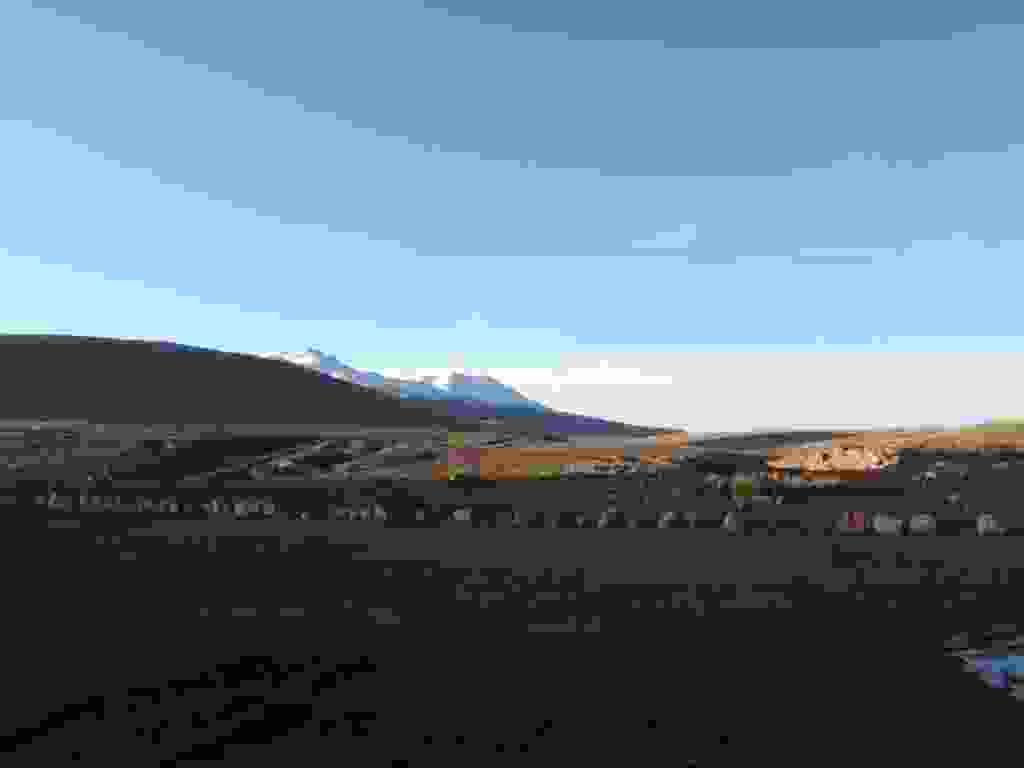
\includegraphics[width=\mywidth]{../wp-content/uploads/2015/03/P3172902-1024x768.jpg} \end{center}
\vfill
\begin{center} 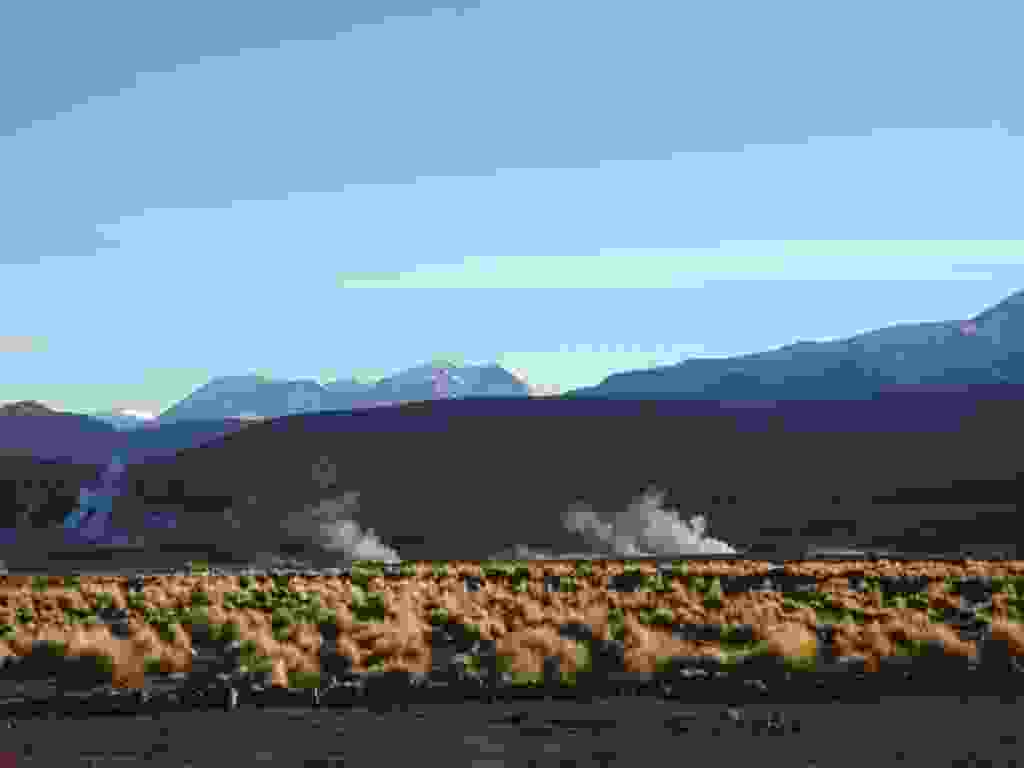
\includegraphics[width=\mywidth]{../wp-content/uploads/2015/03/P3172903-1024x768.jpg} \end{center}
\vspace{-\topsep}
\vspace{-0.75mm}

\pagebreak
 Puis c'est la descente : 90km de 4200m à 2500m pour rejoindre San Pedro de Atacama. 
\begin{center} 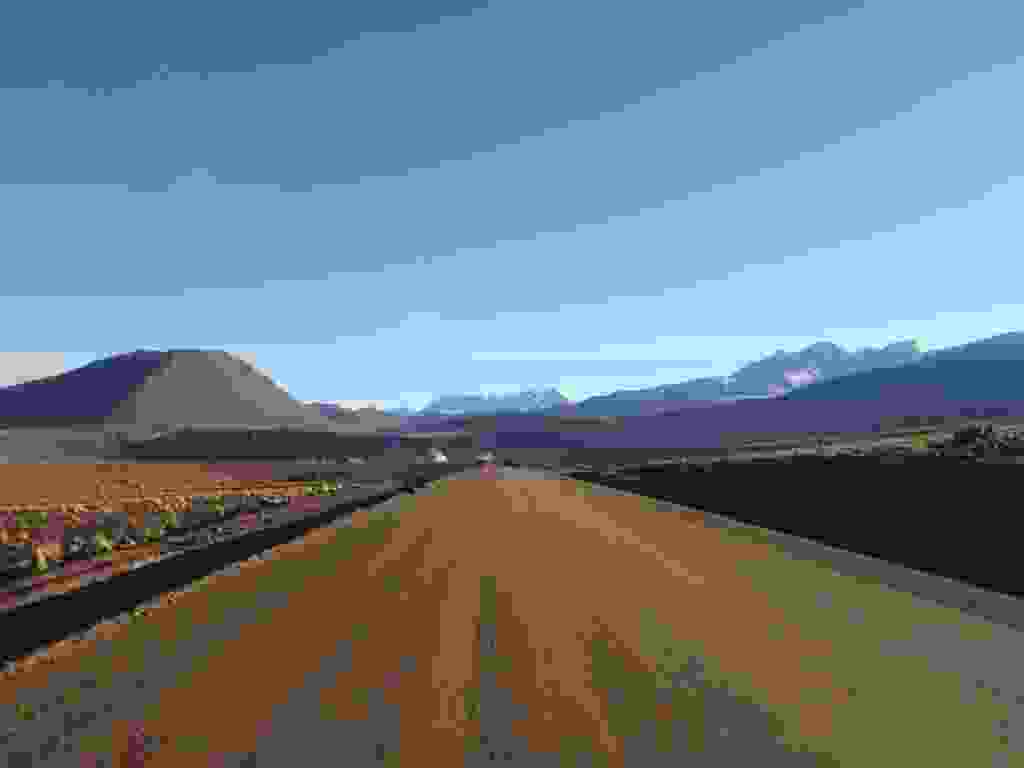
\includegraphics[width=\mywidth]{../wp-content/uploads/2015/03/P3172904-1024x768.jpg} \end{center}
~
\begin{center} 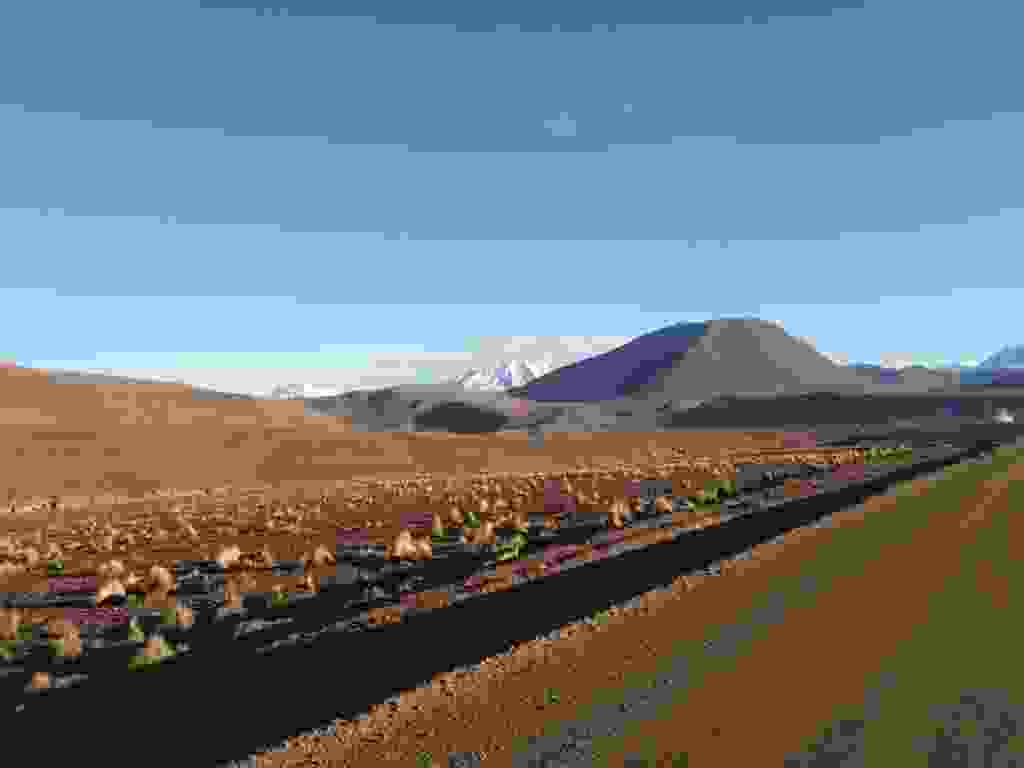
\includegraphics[width=\mywidth]{../wp-content/uploads/2015/03/P3172905-1024x768.jpg} \end{center}
\vspace{-\topsep}
\pagebreak
~\\
\vspace{0.5mm}
\begin{center} 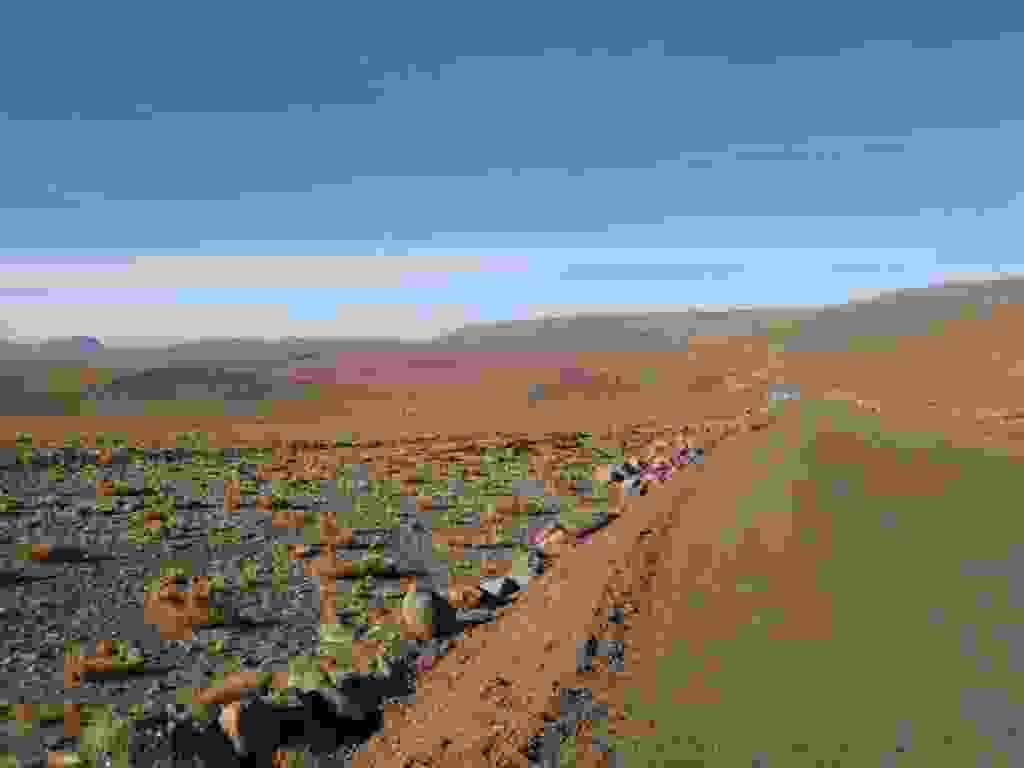
\includegraphics[width=\mywidth]{../wp-content/uploads/2015/03/P3172908-1024x768.jpg} \end{center}

 Je croise régulièrement des vigognes.
\begin{center} \includegraphics[width=\mywidth]{../wp-content/uploads/2015/03/P3172909-1024x768.jpg} \end{center}
\begin{center} \includegraphics[width=\mywidth]{../wp-content/uploads/2015/03/P3172911-1024x768.jpg} \end{center}
\begin{center} \includegraphics[width=\mywidth]{../wp-content/uploads/2015/03/P3172912-1024x768.jpg} \end{center}
\begin{center} \includegraphics[width=\mywidth]{../wp-content/uploads/2015/03/P3172919-1024x768.jpg} \end{center}
\vfill
\begin{center} \includegraphics[width=\mywidth]{../wp-content/uploads/2015/03/P3172922-1024x768.jpg} \end{center}
\vspace{-\topsep}
\vspace{-0.75mm}

\pagebreak
 Le désert d'Atacama au loin. 
\begin{center} \includegraphics[width=\mywidth]{../wp-content/uploads/2015/03/P3172925-1024x768.jpg} \end{center}

 \`A San Pedro je suis hébergé en Warmshowers chez Carlos, en compagnie d'un couple de voyageurs à vélo français Frédéric et Lucie. Quelques jours de repos bien sympathiques. 
\begin{center} \includegraphics[width=\mywidth]{../wp-content/uploads/2015/03/P3172927-1024x768.jpg} \end{center}
\vspace{-\topsep}
\pagebreak
~
\vspace{3mm}
\begin{center} \includegraphics[width=\mywidth]{../wp-content/uploads/2015/03/P31829291-1024x768.jpg} \end{center}

J'attaque bientôt le sud de la Bolivie, une région plutôt isolée, le prochain article ne sera pas pour tout de suite.

 Et merci à tous pour les commentaires, ça m'encourage bien !
